% This file compiles with both LuaLaTeX and XeLaTeX
\documentclass[11pt]{article}

% Change "review" to "final" to generate the final (sometimes called camera-ready) version.
% Change to "preprint" to generate a non-anonymous version with page numbers.
\usepackage[preprint]{acl}

% This is not strictly necessary, and may be commented out,
% but it will improve the layout of the manuscript,
% and will typically save some space.
 \usepackage{microtype}
\usepackage{graphicx}
\usepackage{longtable}
\usepackage{float} % for [H] placement to avoid float overlap
\usepackage{placeins} % optional barriers if needed
% (two-column strip/caption packages removed for single-column layout)
% Tighter float handling and placement on the same page
\setcounter{topnumber}{3}
\setcounter{totalnumber}{5}
\renewcommand{\topfraction}{0.95}
\renewcommand{\textfraction}{0.05}
\renewcommand{\floatpagefraction}{0.9}
\setlength{\textfloatsep}{8pt plus 2pt minus 2pt}
\setlength{\intextsep}{6pt plus 2pt minus 2pt}
\setlength{\abovecaptionskip}{3pt}
\setlength{\belowcaptionskip}{3pt}

% Fixed-width A/C/U formatting for aligned columns within a cell
\newcommand{\ACU}[3]{\makebox[2.0em][r]{#1}/\makebox[2.0em][r]{#2}/\makebox[2.0em][r]{#3}}
\newcommand{\ACUNA}{\makebox[2.2em][c]{-}/\makebox[2.2em][c]{-}/\makebox[2.2em][c]{-}}

% These font selection commands work with
% LuaLaTeX and XeLaTeX, but not pdfLaTeX.
\usepackage[english,bidi=default]{babel} % English as the main language.


\title{\textbf{S}eamlessly Aligning \textbf{L}LMs with \textbf{O}nline User \textbf{P}references (S.L.O.P.) for Creative Generation}


\author{Einar Balan}

\begin{document}

\maketitle
\begin{abstract}
    Current alignment methods for large language models (LLMs)—e.g., RLHF and DPO—optimize for broad consensus, but this limits performance on creative tasks where individual taste is essential. I present S.L.O.P., a framework for scalable personalization in creative generation. My main contribution is a systematic study of soft prompts as a middle ground between resource-heavy fine-tuning and weak prompt-engineering baselines. Using Reddit-derived datasets, I show that soft prompts achieve strong adherence to user preferences and greater output diversity, elevating smaller models (Gemma-3-4B) toward parity with much larger models, with as few as 20-100 training examples. Objective metrics (embedding variance, cosine similarity) confirm these findings, while qualitative analysis highlights trade-offs in coherence at scale. A secondary contribution is a proof-of-concept platform integrating the explored LLM alignment methods directly with a seamless preference collection system. Together, these results demonstrate that lightweight, scalable personalization can make LLMs viable tools for subjective creative generation.
\end{abstract}

% contrinutons include topic categorized reddit train datasets, proposal for new personalization framework for creative generation, extensive, data driven personalizaton testing

\section{Introduction}

% The current state of creative generation, both by humans and LLMs, attempts to create content that is as broadly palatable as psosible. It's clear why this is. The more people that enjoy a work, the (ostensibly) more successful it is. It's impossible to please everyone, so we'll just settle on most. That's good enough. For obvious reasons, in attempting to please as many people as possible, creativity is often stifled and the resulting work is often more muted. 

% idea: take the mathematician's lament approach

% present a world where all creative works try to cater to the masses as much as possible. why do we expect an LLM to be able to produce quality content under the same conditions?

An author wakes up from a terrible nightmare.  In his dream he finds himself in a society where all of his work \emph{must} cater to the widest possible audience. 

He is no longer permitted to fill \emph{his} niche, to think about things that \emph{he} enjoys, or write about what brings \emph{him} satisfaction. Something like that would never succeed! No, he must take care to inform himself on what is currently popular, adjust his own style accordingly, and never deviate beyond the safety of conformity.

His latest work is a new installment in the DCU (Depersonalized Cinematic Universe), featuring appearances from fan favorites like Captain Uninspired, The Homogenizer, and Generic Joe. It will be met with lukewarm response, but a warm one nonetheless \cite{lockhartslament}. 

Thankfully, we don't live in this world. After all, what is the point of art if not to be unique, interesting, and thought provoking? Unfortunately, it does represent what is essentially the current state of creative generation research in LLMs. These models are trained on mountains of content in an effort to gather an understanding of language and the world it describes, and it's clear that this approach has been highly effective for objective applications -- things that have a correct answer. There are hundreds of benchmarks out there to prove it. However, the second you try a more subjective task, like creative writing, poetry, or comedy, the cracks start to show. It's very clear why: through various training methods like RLHF and DPO, the models learn to cater to everybody. For creative tasks, that just won't work.

In order to address this, I have tried to design a scalable method for aligning an LLM as closely as possible with an \emph{individual's} preferences. To me, it seems that there are two critical aspects of this:

\begin{enumerate}
    \item \textbf{Scalability}: It should be feasible to apply the personalization method at scale.
    \item \textbf{Seamless Preference Collection}: It should be easy to collect reliable user preferences towards personalization.
\end{enumerate}

In this work, I'll mostly address the first point, but I will touch on the second as well. To address the first, I'll explore and test a few different personalization methods.

% what makes art interesting is the personal aspect of it. what it represents beyond the face value. if we can find a way to add that personal aspect into LLM generation, it is far more likely to be effective

\section{Related Work}

The initial inspiration to investigate creative generation in LLMs came from \citet{jentzsch2023chatgptfunfunnyhumor}. They showcase the difficulty LLMs have with generating humorous content and some common pitfalls (repeating memorized jokes, nonsensical punchlines, etc). 

This project is most heavily inspired by \citet{ning2024userllm}, which aims to efficiently contextualize LLMs through the use of user embeddings. These embeddings are essentially tokens that uniquely identify a user and their conversation history. In effect, the LLM is provided with a space efficient representation of that user's conversation history, allowing for personalization of future output. The paper takes two approaches: one utilizing cross attention and the other utilizing soft prompts (also known as prompt tuning) to integrate the user embedding with the LLM. This same approach is also discussed in \citet{doddapaneni2024userembeddingmodelpersonalized}. In the case of these works, the user embedding encodes plaintext preferences, such as restaurant ratings. These ratings can then be accessed via the embedding and used to generate recommendations for new restaurants. \citet{liu2024llmspersonaplug} discusses a similar method. 

Soft prompts are investigated in more depth in \citet{lester2021powerscaleparameterefficientprompt} as well as \citet{hebert2024persomapersonalizedsoftprompt}. Briefly, a soft prompt is a prefix optimized through gradient descent that is appended to a prompt at inference time. Critically, many different soft prompts can be applied to a single LLM with minimal effort and resources.

A paper from \citet{richardson2023integratingsummarizationretrievalenhanced} discusses using automatic preference summarization techniques for personalization.


\section{Approach}

I'm proposing a new framework for creative generation that allows for personalization to individual tastes, with an emphasis on scalability and seamless preference collection.

Ultimately, this framework will require an environment similar to those seen in platforms like Reddit, Netflix, TikTok, etc. These platforms are the ultimate preference collection machines, with user preferences being collected as a simple byproduct of using the platform. These preferences provide signficant insight into each user's cultural background and, if utilized correctly, could be integral to generating new content tailored to them. 

To that end, I have built a simple proof of concept application that mimics this environment (though that is not the focus of this work). The preference collection mechanism is essential, but if there is not an effective personalization method then all of that will go to waste. Significant effort has gone into designing, implementing, and thoroughly testing several personalization methods.

\subsection{Personalization Methods}

To be successful in this application, a personalization method needs a few qualities:

\begin{enumerate}
    \item \textbf{Lightweight}: As the method will be applied for many different users, a resource intensive process is not ideal.
    \item \textbf{Flexible}: It should be easy to add and remove personalization from an LLM.
    \item \textbf{Effective}: The method should produce content that adheres to the user's preferences and is generally coherent.
\end{enumerate}

The first and second points immediately rule out finetuning as a personalization strategy and suggest an inference time approach is more appropriate. Unfortunately, inference time strategies (particularly prompt based approaches) are known to be far less effective than finetuning. Is there a happy medium between the two?

Soft prompts appear to meet that happy medium. They are lightweight (in comparison to fine tuning), requiring very limited training data, and very flexible in that many different soft prompts can be applied to the same model at inference time. See related work for more information on soft  prompts.  

In order to determine how effective a soft prompting approach would be, I ran extensive, data driven experiments outlined in the next section.

\section{Experiments}

Effectiveness and resource efficiency of personalization techniques seem to be in tension with each other. Ostensibily, soft prompts occupy the midpoint between these two, satisfying both. It's clear that they are lightweight, but the effectiveness will be detailed in the coming section. In particular, there are a few concrete qualities required for a personlization method to be considered effective:

\begin{enumerate}
    \item \textbf{Adherence}: A majority of the content generated via the method must adhere to the preferences provided.
    \item \textbf{Coherence}: The content generated must be intelligible and limit hallucinations.
    \item \textbf{Variety}: The personalized model should be able to generate a wide range of content, rather than simple variations of the same text repeatedly.
\end{enumerate}

It's useful to have a standard of comparison for the soft prompt approach, so we will also consider the following prompting strategies:

\begin{itemize}
    \item Self Defined: The model is given a manually created description of topics of interest.
    \item Auto-summarized: The model is given an LLM generated summary of a list of posts that adhere to preferences.
    \item Preference History: The model is given direct access to a list of posts that adhere to preferences. 
\end{itemize}

You can see examples of the prompts for these strategies in Appendix A. Each of these satisfy the first two criteria of an effective personalization method: they are very lightweight and flexible. In theory, they are not as effective as the soft prompting approach.

For soft prompting, I first test the ideal size of the training set to make sure we are training effectively. Then I move on to testing each of the personalization strategies.

\subsection{Datasets}

All of the preference data was sourced from Reddit. Much of this was gathered from a \href{https://www.kaggle.com/datasets/noahpersaud/reddit-submissions-dec-2022-to-feb-2023}{Kaggle dataset} (which required extensive cleaning and filtering) and some of it was gathered directly from Reddit using one of their public endpoints. 

I then categorized these posts into various topics of interest such as nerdy posts, posts about parenting, posts about UCLA, in order to then build a "profile" of sorts that could represent the interests of a user. All categorized data can be found \href{https://github.com/EinarBalan/slop/tree/main/datasets}{here}.

The categories of particular interest are: \emph{minecraft, ucla, nostupidquestions, copypasta, nerdy, personal, pop, religion, tech, finance, amitheasshole, okbuddy, food, animals, pregnancy, parenting, baby, boomerhumor}. The contents of each of these is described in more detail in Appendix B.

There are also several "supercategories" consisting of posts from a few categories:
\begin{itemize}
    \item unalike: posts from very different categories (pop, religion, tech)
    \item alike: posts from similar categories (tech, nerdy, finance)
    \item formatspecific: posts from categories that all follow a specific format (copypasta, nostupidquestions, amitheasshole)
    \item college: posts meant to mimic the interests of the stereotypical college student (ucla, nerdy, okbuddy, copypasta, pop, food, animals)
    \item newmother: posts meant to mimic the interests of the stereotypical new mother (pregnancy, parenting, baby, food, amitheasshole, pop, boomerhumor)
\end{itemize}

\subsection{Soft Prompt Train Size Ablation}

I tested across three axes: model size, dataset, and training set size. I opted for gemma-3-4b-it and gemma-3-27b-it for the models.

For the datasets, I stuck to categories focused on single topics. In particular: minecraft, ucla, nostupidquestions, and copypasta. Each of these datasets are very different from each other and provided useful information on how to train the overall best softprompt. The minecraft dataset is ultraspecific to a single game. It's very obvious if a model has been personalized to that interest. The ucla dataset is a bit more broad, but still quite specific to the interests of someone attending UCLA. The nostupidquestions dataset is quite broad but mainly tests stylistic adherence. Each of the posts in that dataset adhere to a very specific format and style. Finally, the copypasta dataset is more of a wild card. Many of the posts are quite incoherent, putting a lot of strain on the soft prompt to adhere to a very niche writing style and set of interests. 

Finally, I tested across training sets of size 10, 20, 50, 100, 250, 500, 1000, and 2000. 

Due to a lack of resources, I did not systematically analyze the posts here, instead opting for a qualititative approach. My finding was that, across the board 100 posts was enough to train a soft prompt with good adherence. Even further, for some of the more targeted datasets such as minecraft, ~20 posts was all that was needed. This shows the significant benefit of soft prompts over fine tuning: they are significantly less resource intensive.

\subsection{Personalization Strategies Ablation}

Similarly to above, I tested across three axes here: model size, dataset, and personalization method. For the soft prompt training set, I included 100 posts as determined above. 

For these experiments, I used gemma-3-4b-it, gemma-3-27b-it, and gpt-5. I could not test the soft prompt approach on gpt-5 as I only have access to the API, but it served as a useful standard of comparison for the prompt based approaches. In particular, I was interested to see how model size affected adherence, coherence, and variety of generated posts across the different datasets and personalization strategies. Note that I used the same hyperparameters (when applicable) including a temperature of 0.7 and top p sampling method with p = 0.9. I also added a repetition penalty of 1.1.

For the datasets, I used nerdy, personal, unalike, alike, format specific, college, and newmother. More information on datasets can be found in Appendix B.

As discussed earlier, the personalization methods include soft prompts, self defined interests, auto-summarized interests, and a list of posts exhibiting interests (which I will refer to as like history from this point).

\subsubsection*{Soft Prompt Training Process}

As discussed, I settled on a training set size of 100 posts for each dataset. Each soft prompt consists of 64 tokens and I trained with a learning rate of 0.2 and a maximum of 1000 training steps. Note the steep learning rate, which is required to training soft prompts effectively.

\subsection{Results}

\begin{figure}[t!]
    \centering
    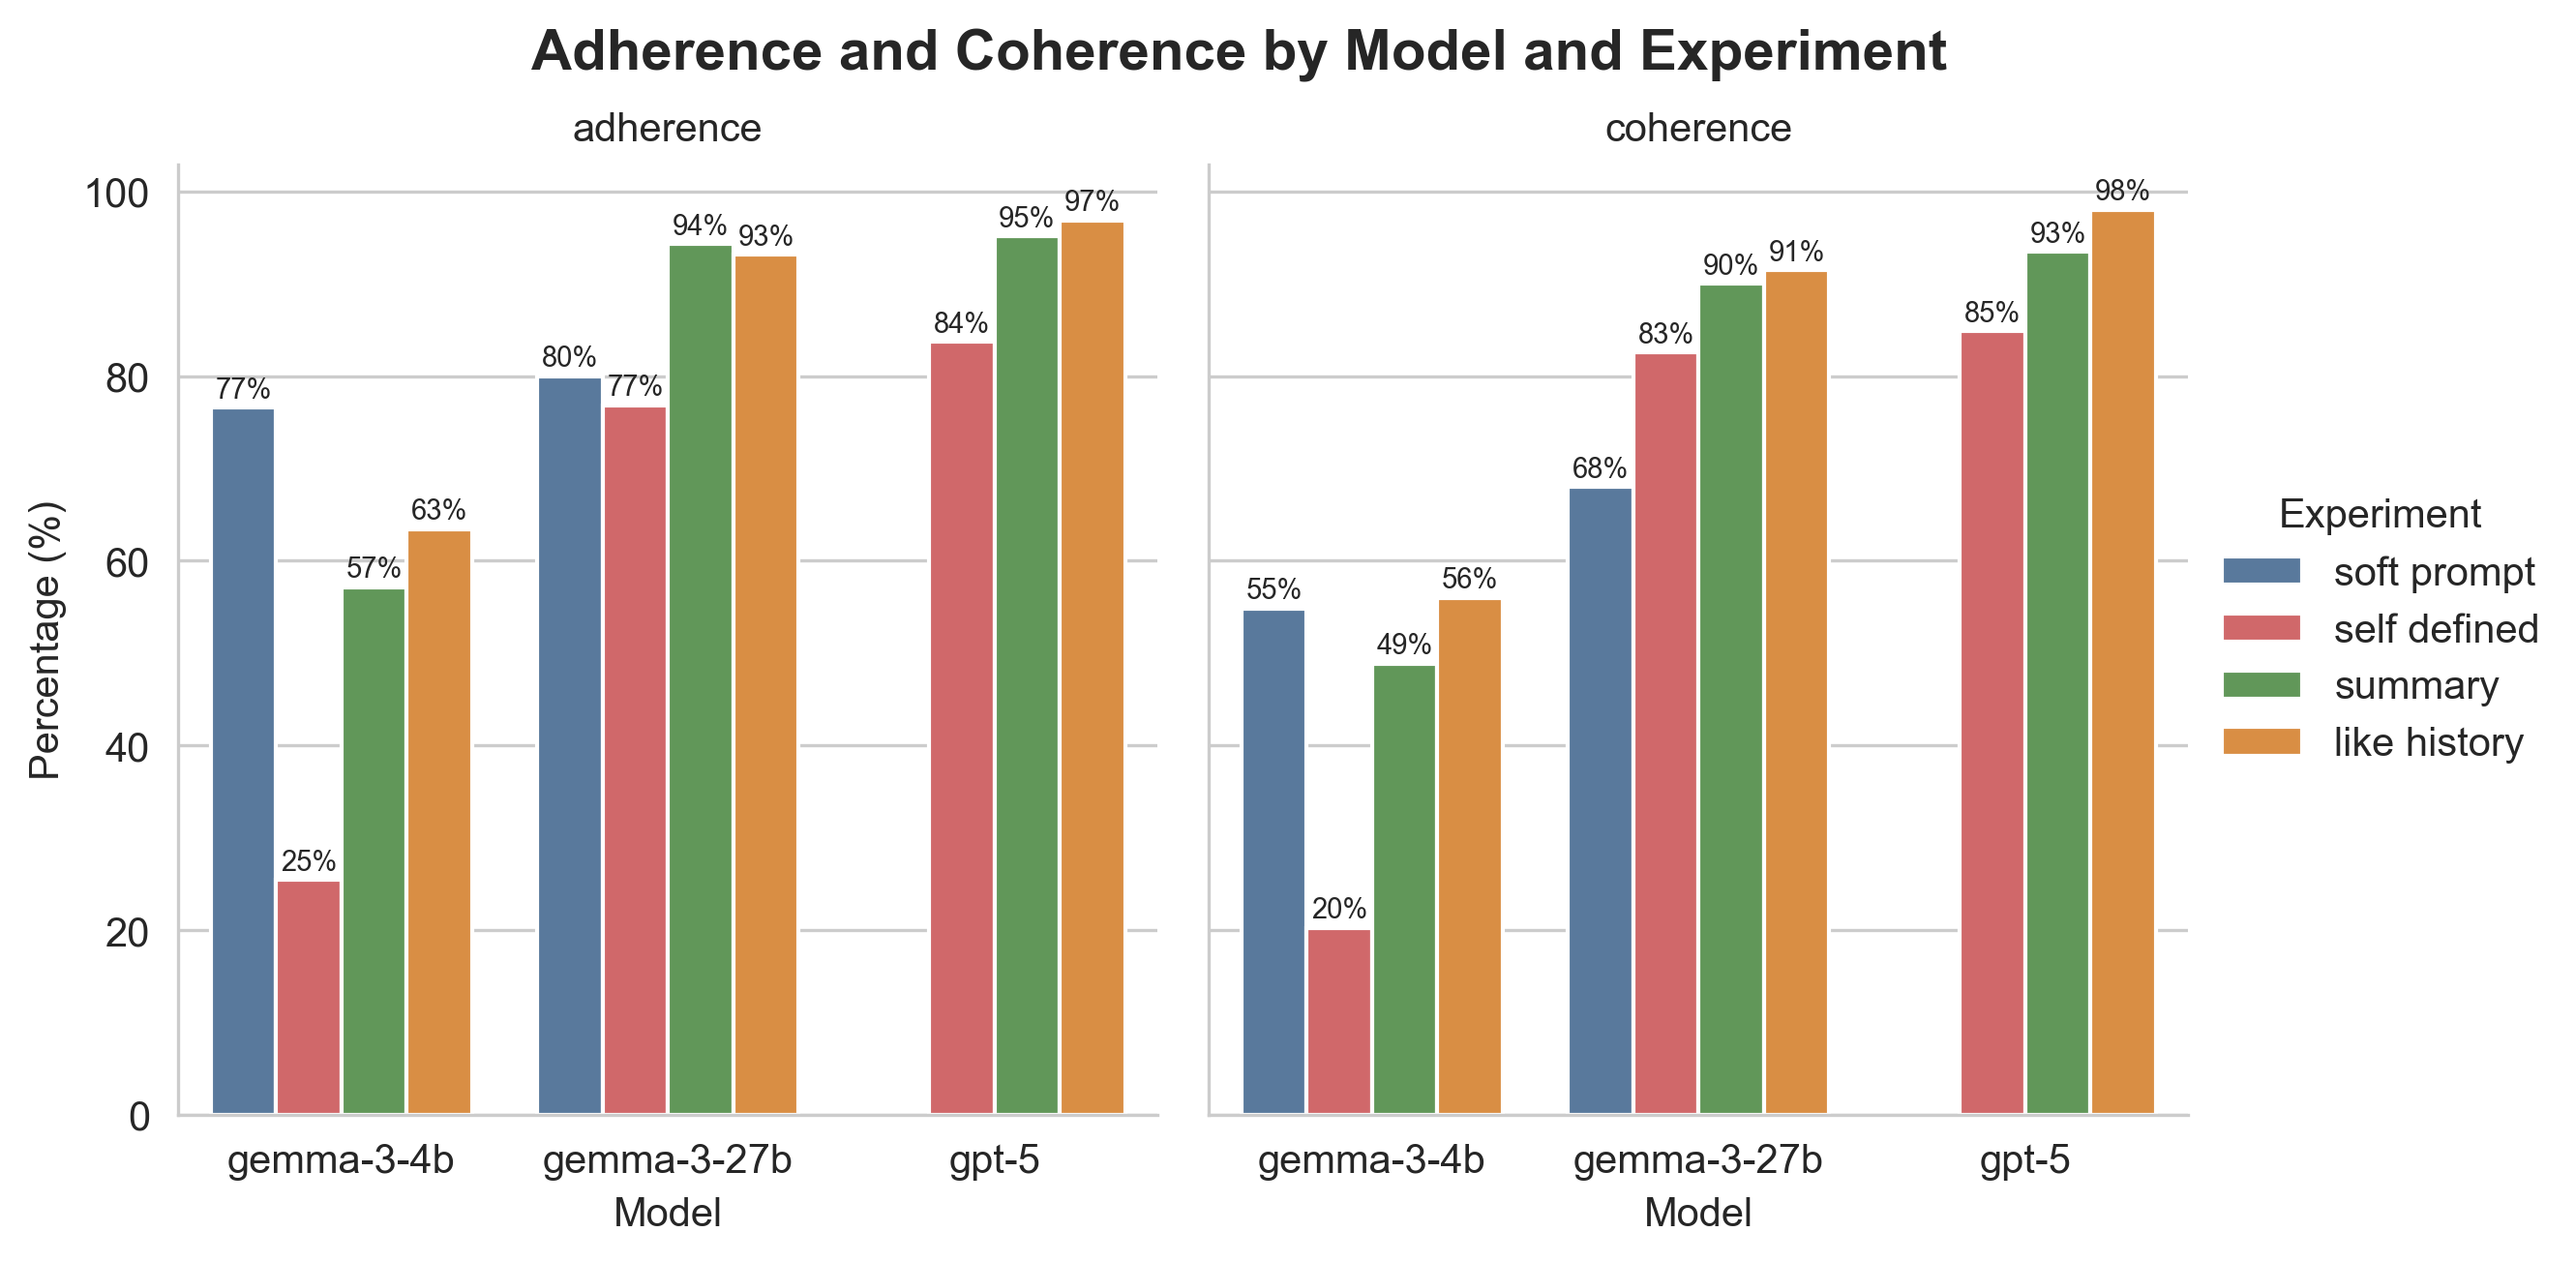
\includegraphics[width=\linewidth]{visuals/acu-by-model-experiment.png}
    \caption{Adherence refers to how closely the generated output adheres to the provided preferences and coherence refers to the intelligibility of the text. Note that there was no soft prompt experiment for gpt-5.}
    \label{fig:acu-rates}
    \end{figure}

\begin{figure}[t!]
\centering
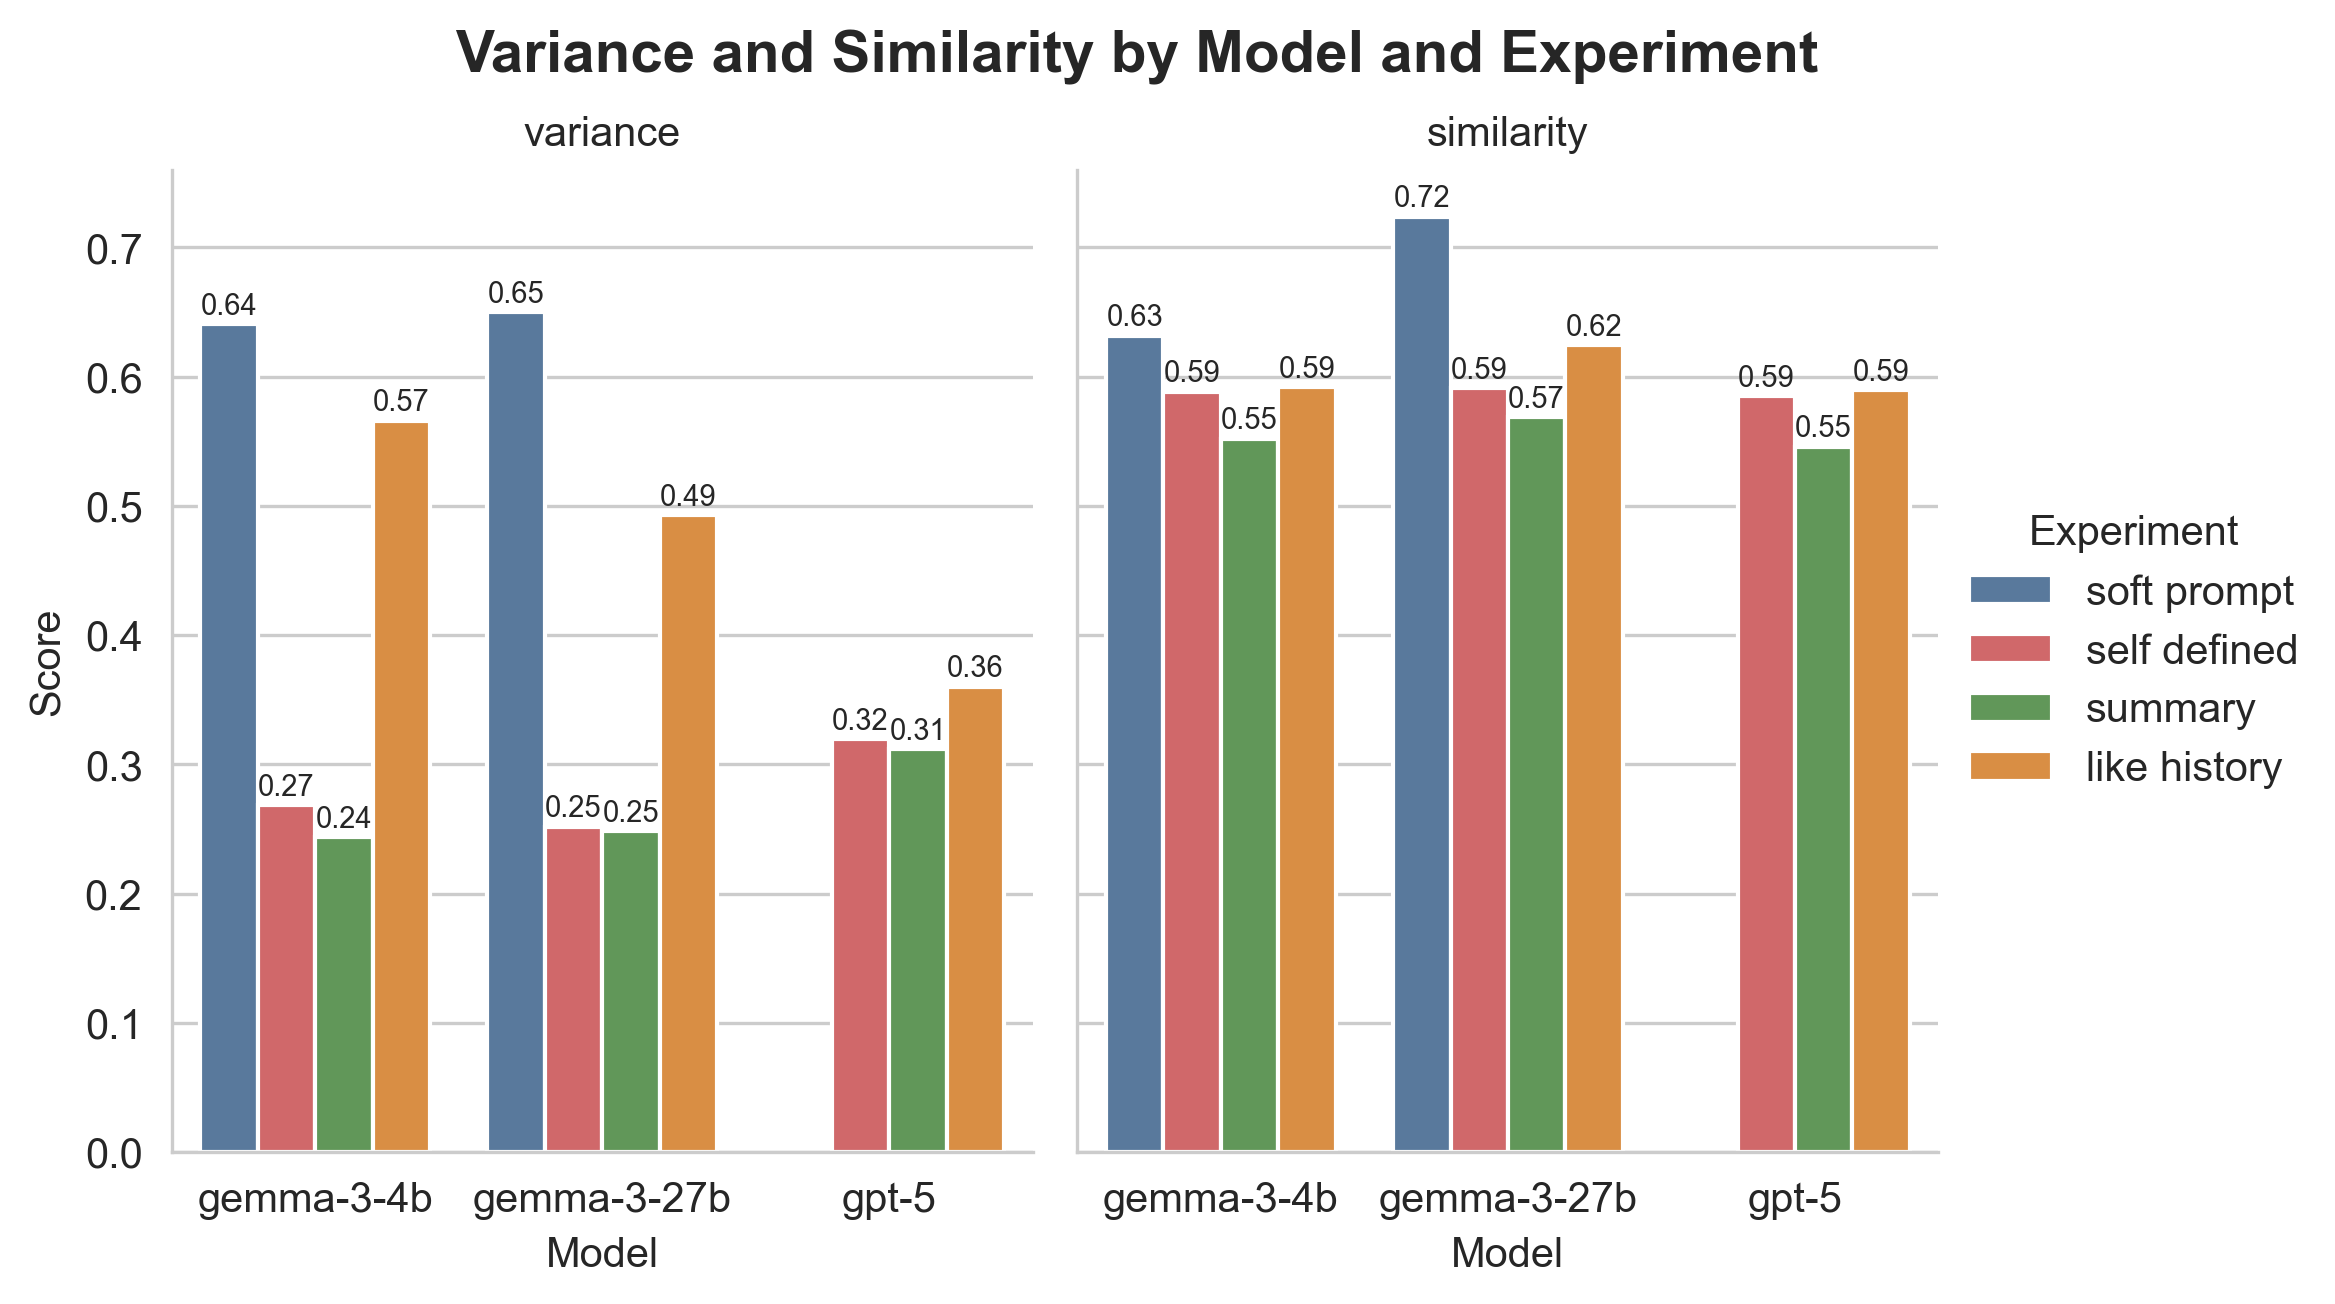
\includegraphics[width=\linewidth]{visuals/variance-similarity-by-model-experiment.png}
\caption{Variance measures the variability of the embeddings of the posts generated through a personalization strategy and similarity measures the cosine similarity of the mean embedding of the original dataset to the mean embedding of the generated posts. For each, higher is better.}
\label{fig:variance-similarity}
\end{figure}


Effectiveness of a personalization method comes down to three qualities: adherence, coherence, and variety. Figure~\ref{fig:acu-rates} shows the adherence and coherence rates grouped by model and personalization strategy. Interestingly, we see the soft prompt approach vastly outperforms the prompt based approaches for the smaller model on adherence, but lags behind for the 27b model. This suggests that the larger a model gets, the better its abiliy to interpet user's intent behind a prompt, leading to better adherence results. 

Coherence showed a similar story, with the soft prompt approach being about on par with like history, but far outperforming the other 2 moethods on the 4b model. It also lags behind for the 27b model. These results are quite encouraging, because they show that a soft prompt can be used to bring the performance of a much smaller model to around the same level as a larger model. Coherence struggles a bit on the 27b model, but it's likely this is a training issue.

It should be noted that the adherence and coherence data was all manually labeled (approx. 4000 posts). The labeler (me) didn't know which experiment each post belonged to, so no bias was in play there. Clearly, manually labeled data is not ideal, so we also include some objective metrics, namely embedding variance and cosine similarity to the original dataset. The embedding model used is sentence-transformers/all-MiniLM-L6-v2. 

Embedding variance is useful to determine how much variety the personalization strategy is able to produce in its dataset. The larger variety of topics and styles we can produce, while still adhering to preferences and staying coherent, the better. Variance is useful to pinpoint a single number, but a visual approach can be helpful. To this end, I also clustered the embeddings for each approach to see how widely spread they are. These can be found in Appendix D. Ideally, we want minimal clustering for this application. A cluster usually indicates that a personalization strategy is producing many variants of the same post with minimal changes. It's possible that all these variants adhere to the preferences and are coherent, but the large quantity of variants produced unfairly inflates the adherence and coherence numbers. Therefore, it is important to take into account the variance and clustering numbers as well. We should note that for every model, the soft prompt approach produces the highest variety and lowest number of clusters. Every other approach suffers from low variety to some degree.

The cosine similarity metric serves a similar function to the adherence metric except that it is entirely objective. Interestingly, we see that yet again, the soft prompt approach outperforms all of the other methods, with a larger lead on the 27b model. This is in contrast to the manually gathered adherence results. Overall, these results seem to suggest that soft prompts provide the best personalization in terms of adherence and variety, with coherence struggling a bit. However, for smaller models it is the undisputed winner.

\subsubsection*{Additional Discussion}

Some minor details of note:
\begin{itemize}
    \item soft prompt generation was significantly faster compared to any of the other approaches (though I don't have concrete times)
    \item whenever the models attempted humor, no matter the personalization strategy, the coherence dropped. this is a big reason why the soft prompt approach appears to lack coherence as it attempted humor far more often than the other approaches (when relevant)
    \item stylistically, the soft prompt posts are vastly more similar compared to other approaches. I didn't account for that while labeling, but that is likely why we see the similarity/adherence discrepancy
\end{itemize}

There is a lot more to get into here in terms of fine grained analysis, but we'll omit that here.

\section{Conclusions \& Future Work}

We have shown that soft prompting provides the best all around method for scalable personalization towards creative generation. What remains how is to demonstrate the seamless preference collection process. As mentioned, an environment to do so has been fully implemented and just needs to be tested. This environment would also provide valuable data indicating like rates for AI generated content and how well the content blends into to human generated content. Unforunately, to test it requires a lot of time and resources that I do not currently have. 

The application mimics reddit with the twist that some of the posts served are LLM generated. These generated posts can be produced with any of the personalization mechanism presented here, or even no personalizatio method. As the user uses the app, we naturally collect their preferences for the topics and styles of content they prefer, as well as measure how well a given personalization mechanism performs. The user can interact with a post in three ways: an upvote, a downvote, or a "mark as AI." We can then compare each of the personalization strategies on these three metrics to determine performance.

Additionally, in retrospect some degree of stylistic adherence would have been useful to measure as well. It would also have been nice to automate the coherence metric with an LLM judge, though in my limited time I was not able to produce one with reliable results. With some finetuning and more time, it could be very doable and improve the scalability of the methodolgy. On that note, comparing the personalization methods to fine tuned models could also have been interesting, but again it was challenging to integrate given the time requirements. 

It's clear to me that there is a lot of potential with this work. This is just one small babystep, but I envision a similar approach being utilized for more than just social media post generation. Any creative generation application could benefit: creative writing, video generation, or even music generation. Imagine a Netflix app where you can generate a movie perfectly tailored to your preferences on a whim. That's the potential I see. Clearly these are just baby steps, but it is an exciting direction!

\section{Ethical Considerations}

There is a lot of debate over AI generated art. Many worry that it could devalue human art and place the livelihoods of many artists at risk. I certainly understand that worry. It's one that could be applied to virtually any field. I would argue that art in particular, though, is safe. Most varieties of it, anyway. 

The thing that makes art interesting is the story behind it. The human element. That's something you can't get with a solely AI generated work. There will always be something missing and it won't feel the same. There certainly is a time and a place for AI generated content, but I see it more so as a low stakes time waster, similar to the niche that social media like TikTok currently fills.

It can be uncomfortable to see someone generate an image in seconds that would have taken a human artist hours to create. On the whole, however, I think this is a good thing! It evens the playing field. Anyone can be an artist. Anyone can express themselves. As always, the good art will be recognized and the bad will be cast aside (in so far as there even is such a thing as good and bad art). Ultimately, I think it will be a net positive.

% Entries for the entire Anthology, followed by custom entries
\bibliography{custom}

\clearpage

\appendix

\section{Appendix: Prompts}

\begin{longtable}{|p{3cm}|p{10cm}|}
\caption{Personalization Strategy Prompts}\\
\hline
\textbf{Personalization Strategy} & \textbf{Prompt} \\
\hline
Like History & Please generate one reddit post similar to the following posts:
title: I need a Chrons friendly, gluten free, and only hard cheeses recipe.
self\_text: A buddy of mine has a lot of digestive issues and he's never really had anyone cook for him so I wanted to treat him. I want something fancy as hell and I'm not worried about price of ingredients at all. I want something that's really gonna blow him away and impress him. I know he can eat chicken and any seafood but like selfish do give him a minor reaction. Red meat is completely off the table.
subreddit: Cooking [...] It is critical that you stick to this exact format. DO NOT ADD ANYTHING ELSE. \textbackslash n\textbackslash ntitle: \{title\}\textbackslash n self\_text: \{self\_text\}\textbackslash n subreddit: \{subreddit\}
 \\
\hline
Self Defined & Please generate one reddit post. Here are some topics of interest: gaming, pcs, tech, mmos, rpgs, anime. Pick exactly ONE topic per post. It is critical that you stick to this exact format. DO NOT ADD ANYTHING ELSE. \textbackslash n\textbackslash ntitle: \{title\}\textbackslash n self\_text: \{self\_text\}\textbackslash n subreddit: \{subreddit\} \\
\hline
Soft Prompt & Please generate one reddit post. It is critical that you stick to this exact format. DO NOT ADD ANYTHING ELSE. \textbackslash n\textbackslash ntitle: \{title\}\textbackslash n self\_text: \{self\_text\}\textbackslash n subreddit: \{subreddit\} \\
\hline
Summary & Please generate one reddit post. Here is a summary of the user's interests: Here’s a concise profile of interests inferred from the posts they liked: - Home cooking and food science: practical technique tips (stainless steel searing, pan sauces), balancing flavors (sweetness/acidity in Middle Eastern dishes), creamy vs béchamel gratins, browned butter hacks, mashed potatoes, pasta salad takes, food safety, and specialty diets (gluten‑free/Crohn’s‑friendly). Also into kitchen tools (tweezers) and bouillon/seasoning ideas. - Pets and pet care: Dogs: durable beds, hypoallergenic breeds for families, washing donut beds, ESA housing rules, puppy training/over‑arousal and separation‑anxiety protocols, gear (bowls), adoption fit (Yorkie‑poodle). Cats: eye/medical issues, UT prescription diets and treat rules, behavior/being held, leash/harness acclimation.  Pick exactly ONE topic per post. It is critical that you stick to this exact format. DO NOT ADD ANYTHING ELSE. title: \{title\} self\_text: \{self\_text\} subreddit: \{subreddit\} \\
\hline
\end{longtable}


\clearpage

\section{Appendix: Datasets}
\label{sec:appendix}

Here's a brief description of each category in the reddit dataset. 

\begin{itemize}
    \item minecraft: posts related to minecraft
    \item ucla: posts related to UCLA and college life in general
    \item nostupidquestions: posts from the subreddit r/NoStupidQuestions, ranging a variety of topics in a specific format
    \item copypasta: posts from the subreddit r/copypasta ranging a wide variety of topics, but often centered around crude humor and repetition
    \item nerdy: posts related to gaming, pc building, anime, and other nerdy interests
    \item personal: posts related to personal issues such as relationship advice and mental health        
    \item pop: posts related to pop culture, tv, movies, sports, etc.
    \item religion: posts related to religion and spirituality
    \item tech: posts related to consumer technology, hardware, and software
    \item finance: posts related to finance, stocks, and investing
    \item amitheasshole: posts related to interpersonal issues, advice
    \item okbuddy: posts related to crude, gen z humor
    \item food: posts related to food, cooking, etc.
    \item animals: posts related to pets, cats, dogs, animals, fish
    \item pregnancy: posts related to pregnancy
    \item parenting: posts related to parenting
    \item baby: posts related to babies
    \item boomerhumor: posts related to traditional jokes e.g. puns, knock knock, etc.
\end{itemize}

\clearpage
\section{Appendix: Metrics Tables}

\begin{table}[H]
\centering
\caption{Adherence/Coherence/Unique for gemma-3-4b-it}
\begin{tabular}{|l|ccc|ccc|ccc|ccc|}
\hline
\textbf{Dataset} & \multicolumn{3}{c|}{\textbf{Soft Prompt}} & \multicolumn{3}{c|}{\textbf{Self Defined}} & \multicolumn{3}{c|}{\textbf{Summary}} & \multicolumn{3}{c|}{\textbf{Like History}} \\
\hline
%  & A & C & U & A & C & U & A & C & U & A & C & U \\
% \hline
nerdy & 88 & 70 & 0 & 2 & 0 & 0 & 26 & 64 & 0 & 90 & 78 & 0 \\
\hline
personal & 74 & 64 & 6 & 48 & 38 & 0 & 52 & 40 & 0 & 42 & 32 & 0 \\
\hline
unalike & 82 & 60 & 6 & 2 & 2 & 0 & 96 & 94 & 0 & 32 & 32 & 0 \\
\hline
alike & 84 & 78 & 44 & 80 & 68 & 0 & 62 & 48 & 0 & 98 & 98 & 14 \\
\hline
formatspecific & 76 & 40 & 2 & 42 & 30 & 0 & 98 & 48 & 0 & 50 & 42 & 0 \\
\hline
college & 78 & 66 & 12 & 0 & 0 & 0 & 2 & 2 & 0 & 64 & 58 & 8 \\
\hline
newmother & 54 & 6 & 2 & 4 & 4 & 2 & 64 & 46 & 0 & 68 & 52 & 4 \\
\hline
\end{tabular}
\end{table}

\begin{table}[H]
    \centering
    \caption{Variance for gemma-3-4b-it}
    \begin{tabular}{|l|c|c|c|c|}
    \hline
    \textbf{Dataset} & \textbf{Soft Prompt} & \textbf{Self Defined} & \textbf{Summary} & \textbf{Like History} \\
    \hline
    alike & 0.666 & 0.188 & 0.175 & 0.463 \\
    \hline
    college & 0.700 & 0.310 & 0.098 & 0.703 \\
    \hline
    formatspecific & 0.673 & 0.269 & 0.250 & 0.630 \\
    \hline
    nerdy & 0.581 & 0.145 & 0.377 & 0.373 \\
    \hline
    newmother & 0.574 & 0.255 & 0.306 & 0.632 \\
    \hline
    personal & 0.590 & 0.632 & 0.391 & 0.538 \\
    \hline
    unalike & 0.702 & 0.080 & 0.108 & 0.623 \\
    \hline
    \end{tabular}
    \end{table}

\begin{table}[H]
    \centering
    \caption{Similarity to Original for gemma-3-4b-it}
    \begin{tabular}{|l|c|c|c|c|}
    \hline
    \textbf{Dataset} & \textbf{Soft Prompt} & \textbf{Self Defined} & \textbf{Summary} & \textbf{Like History} \\
    \hline
    alike & 0.594 & 0.667 & 0.526 & 0.581 \\
    \hline
    college & 0.573 & 0.565 & 0.361 & 0.700 \\
    \hline
    formatspecific & 0.736 & 0.538 & 0.658 & 0.671 \\
    \hline
    nerdy & 0.770 & 0.618 & 0.623 & 0.296 \\
    \hline
    newmother & 0.428 & 0.614 & 0.528 & 0.562 \\
    \hline
    personal & 0.786 & 0.772 & 0.696 & 0.823 \\
    \hline
    unalike & 0.534 & 0.345 & 0.472 & 0.510 \\
    \hline
    \end{tabular}
\end{table}

\clearpage

\begin{table}[H]
\centering
\caption{Adherence/Coherence/Unique for gemma-3-27b-it}
\begin{tabular}{|l|ccc|ccc|ccc|ccc|}
\hline
\textbf{Dataset} & \multicolumn{3}{c|}{\textbf{Soft Prompt}} & \multicolumn{3}{c|}{\textbf{Self Defined}} & \multicolumn{3}{c|}{\textbf{Summary}} & \multicolumn{3}{c|}{\textbf{Like History}} \\
\hline
%  & A & C & U & A & C & U & A & C & U & A & C & U \\
% \hline
nerdy & 86 & 74 & 4 & 98 & 100 & 0 & 78 & 82 & 0 & 94 & 98 & 6 \\
\hline
personal & 86 & 78 & 16 & 100 & 98 & 6 & 98 & 100 & 0 & 100 & 98 & 6 \\
\hline
unalike & 76 & 62 & 8 & 98 & 88 & 4 & 100 & 94 & 2 & 78 & 74 & 2 \\
\hline
alike & 86 & 84 & 14 & 92 & 94 & 2 & 100 & 100 & 0 & 98 & 98 & 20 \\
\hline
formatspecific & 86 & 80 & 6 & 4 & 0 & 0 & 94 & 68 & 2 & 100 & 96 & 6 \\
\hline
college & 82 & 58 & 28 & 46 & 98 & 0 & 100 & 92 & 2 & 84 & 78 & 16 \\
\hline
newmother & 58 & 40 & 18 & 100 & 100 & 0 & 90 & 94 & 0 & 98 & 98 & 6 \\
\hline
\end{tabular}
\end{table}

\begin{table}[H]
    \centering
    \caption{Variance for gemma-3-27b-it}
    \begin{tabular}{|l|c|c|c|c|}
    \hline
    \textbf{Dataset} & \textbf{Soft Prompt} & \textbf{Self Defined} & \textbf{Summary} & \textbf{Like History} \\
    \hline
    alike & 0.633 & 0.269 & 0.217 & 0.587 \\
    \hline
    college & 0.721 & 0.185 & 0.212 & 0.657 \\
    \hline
    formatspecific & 0.739 & 0.312 & 0.229 & 0.355 \\
    \hline
    nerdy & 0.633 & 0.234 & 0.337 & 0.432 \\
    \hline
    newmother & 0.524 & 0.143 & 0.219 & 0.360 \\
    \hline
    personal & 0.575 & 0.294 & 0.204 & 0.401 \\
    \hline
    unalike & 0.726 & 0.325 & 0.321 & 0.658 \\
    \hline
    \end{tabular}
    \end{table}

\begin{table}[H]
    \centering
    \caption{Similarity to Original for gemma-3-27b-it}
    \begin{tabular}{|l|c|c|c|c|}
    \hline
    \textbf{Dataset} & \textbf{Soft Prompt} & \textbf{Self Defined} & \textbf{Summary} & \textbf{Like History} \\
    \hline
    alike & 0.763 & 0.744 & 0.593 & 0.680 \\
    \hline
    college & 0.708 & 0.419 & 0.377 & 0.481 \\
    \hline
    formatspecific & 0.693 & 0.496 & 0.623 & 0.717 \\
    \hline
    nerdy & 0.847 & 0.607 & 0.629 & 0.512 \\
    \hline
    newmother & 0.478 & 0.538 & 0.677 & 0.715 \\
    \hline
    personal & 0.901 & 0.646 & 0.582 & 0.640 \\
    \hline
    unalike & 0.675 & 0.688 & 0.501 & 0.624 \\
    \hline
    \end{tabular}
\end{table}

\clearpage


\begin{table}[H]
\centering
\caption{Adherence/Coherence/Unique for gpt-5}
\begin{tabular}{|l|ccc|ccc|ccc|}
\hline
\textbf{Dataset} & \multicolumn{3}{c|}{\textbf{Self Defined}} & \multicolumn{3}{c|}{\textbf{Summary}} & \multicolumn{3}{c|}{\textbf{Like History}} \\
\hline
%  & A & C & U & A & C & U & A & C & U \\
% \hline
nerdy & 98 & 100 & 0 & 78 & 82 & 0 & 94 & 98 & 6 \\
\hline
personal & 100 & 98 & 4 & 98 & 100 & 0 & 100 & 98 & 4 \\
\hline
unalike & 98 & 88 & 4 & 100 & 98 & 0 & 90 & 100 & 0 \\
\hline
alike & 100 & 100 & 4 & 100 & 100 & 0 & 100 & 100 & 10 \\
\hline
formatspecific & 10 & 10 & 0 & 100 & 80 & 0 & 100 & 96 & 0 \\
\hline
college & 80 & 98 & 0 & 100 & 100 & 0 & 96 & 96 & 4 \\
\hline
newmother & 100 & 100 & 0 & 90 & 94 & 0 & 98 & 98 & 10 \\
\hline
\end{tabular}
\end{table}

\begin{table}[H]
\centering
\caption{Variance for gpt-5}
\begin{tabular}{|l|c|c|c|}
\hline
\textbf{Dataset} & \textbf{Self Defined} & \textbf{Summary} & \textbf{Like History} \\
\hline
alike & 0.152 & 0.093 & 0.265 \\
\hline
college & 0.495 & 0.274 & 0.466 \\
\hline
formatspecific & 0.406 & 0.443 & 0.504 \\
\hline
nerdy & 0.294 & 0.296 & 0.259 \\
\hline
newmother & 0.376 & 0.333 & 0.362 \\
\hline
personal & 0.358 & 0.340 & 0.368 \\
\hline
unalike & 0.157 & 0.402 & 0.298 \\
\hline
\end{tabular}
\end{table}


\begin{table}[H]
\centering
\caption{Similarity to Original for gpt-5}
\begin{tabular}{|l|c|c|c|}
\hline
\textbf{Dataset} & \textbf{Self Defined} & \textbf{Summary} & \textbf{Like History} \\
\hline
alike & 0.653 & 0.634 & 0.692 \\
\hline
college & 0.561 & 0.372 & 0.308 \\
\hline
formatspecific & 0.660 & 0.170 & 0.683 \\
\hline
nerdy & 0.603 & 0.607 & 0.347 \\
\hline
newmother & 0.304 & 0.717 & 0.727 \\
\hline
personal & 0.698 & 0.662 & 0.750 \\
\hline
unalike & 0.617 & 0.658 & 0.620 \\
\hline
\end{tabular}
\end{table}

\clearpage
\section{Appendix: Charts}

\begin{figure}[h]
    \centering
    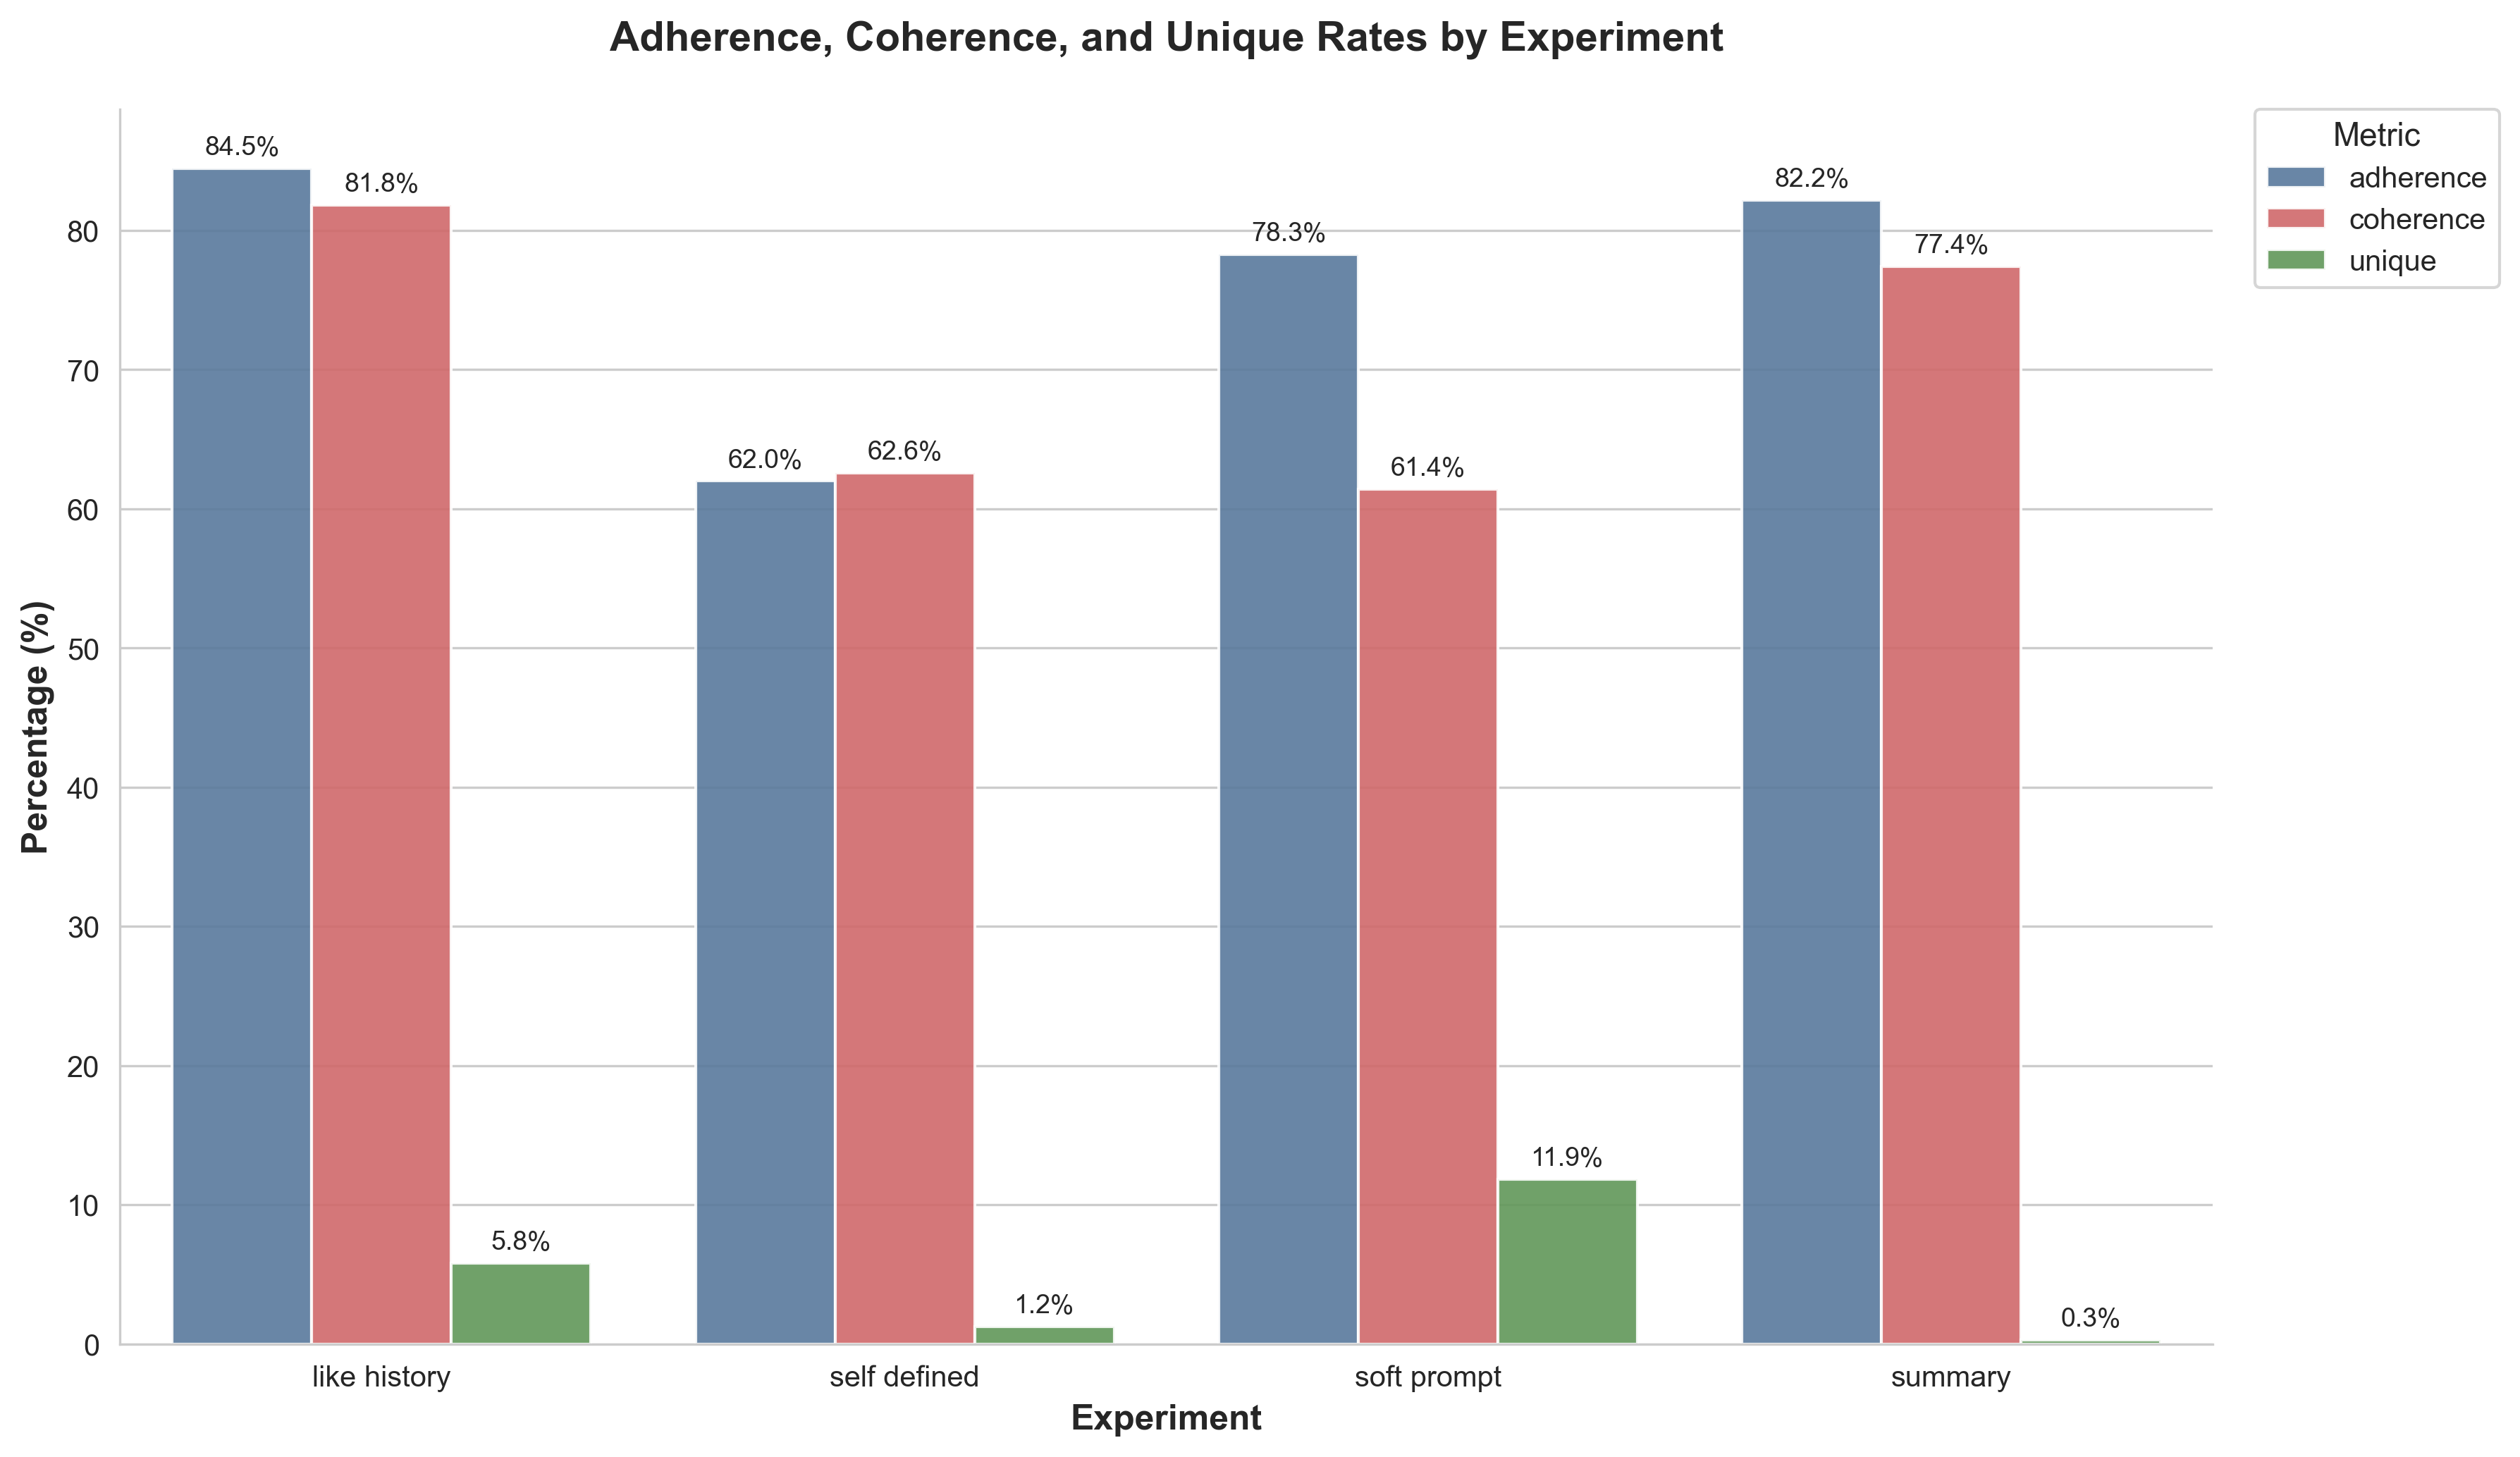
\includegraphics[width=\linewidth]{visuals/acu-rates.png}
    \caption{}
    \label{fig:clustering-gemma-3-4b}
\end{figure}

\begin{figure}[h]
    \centering
    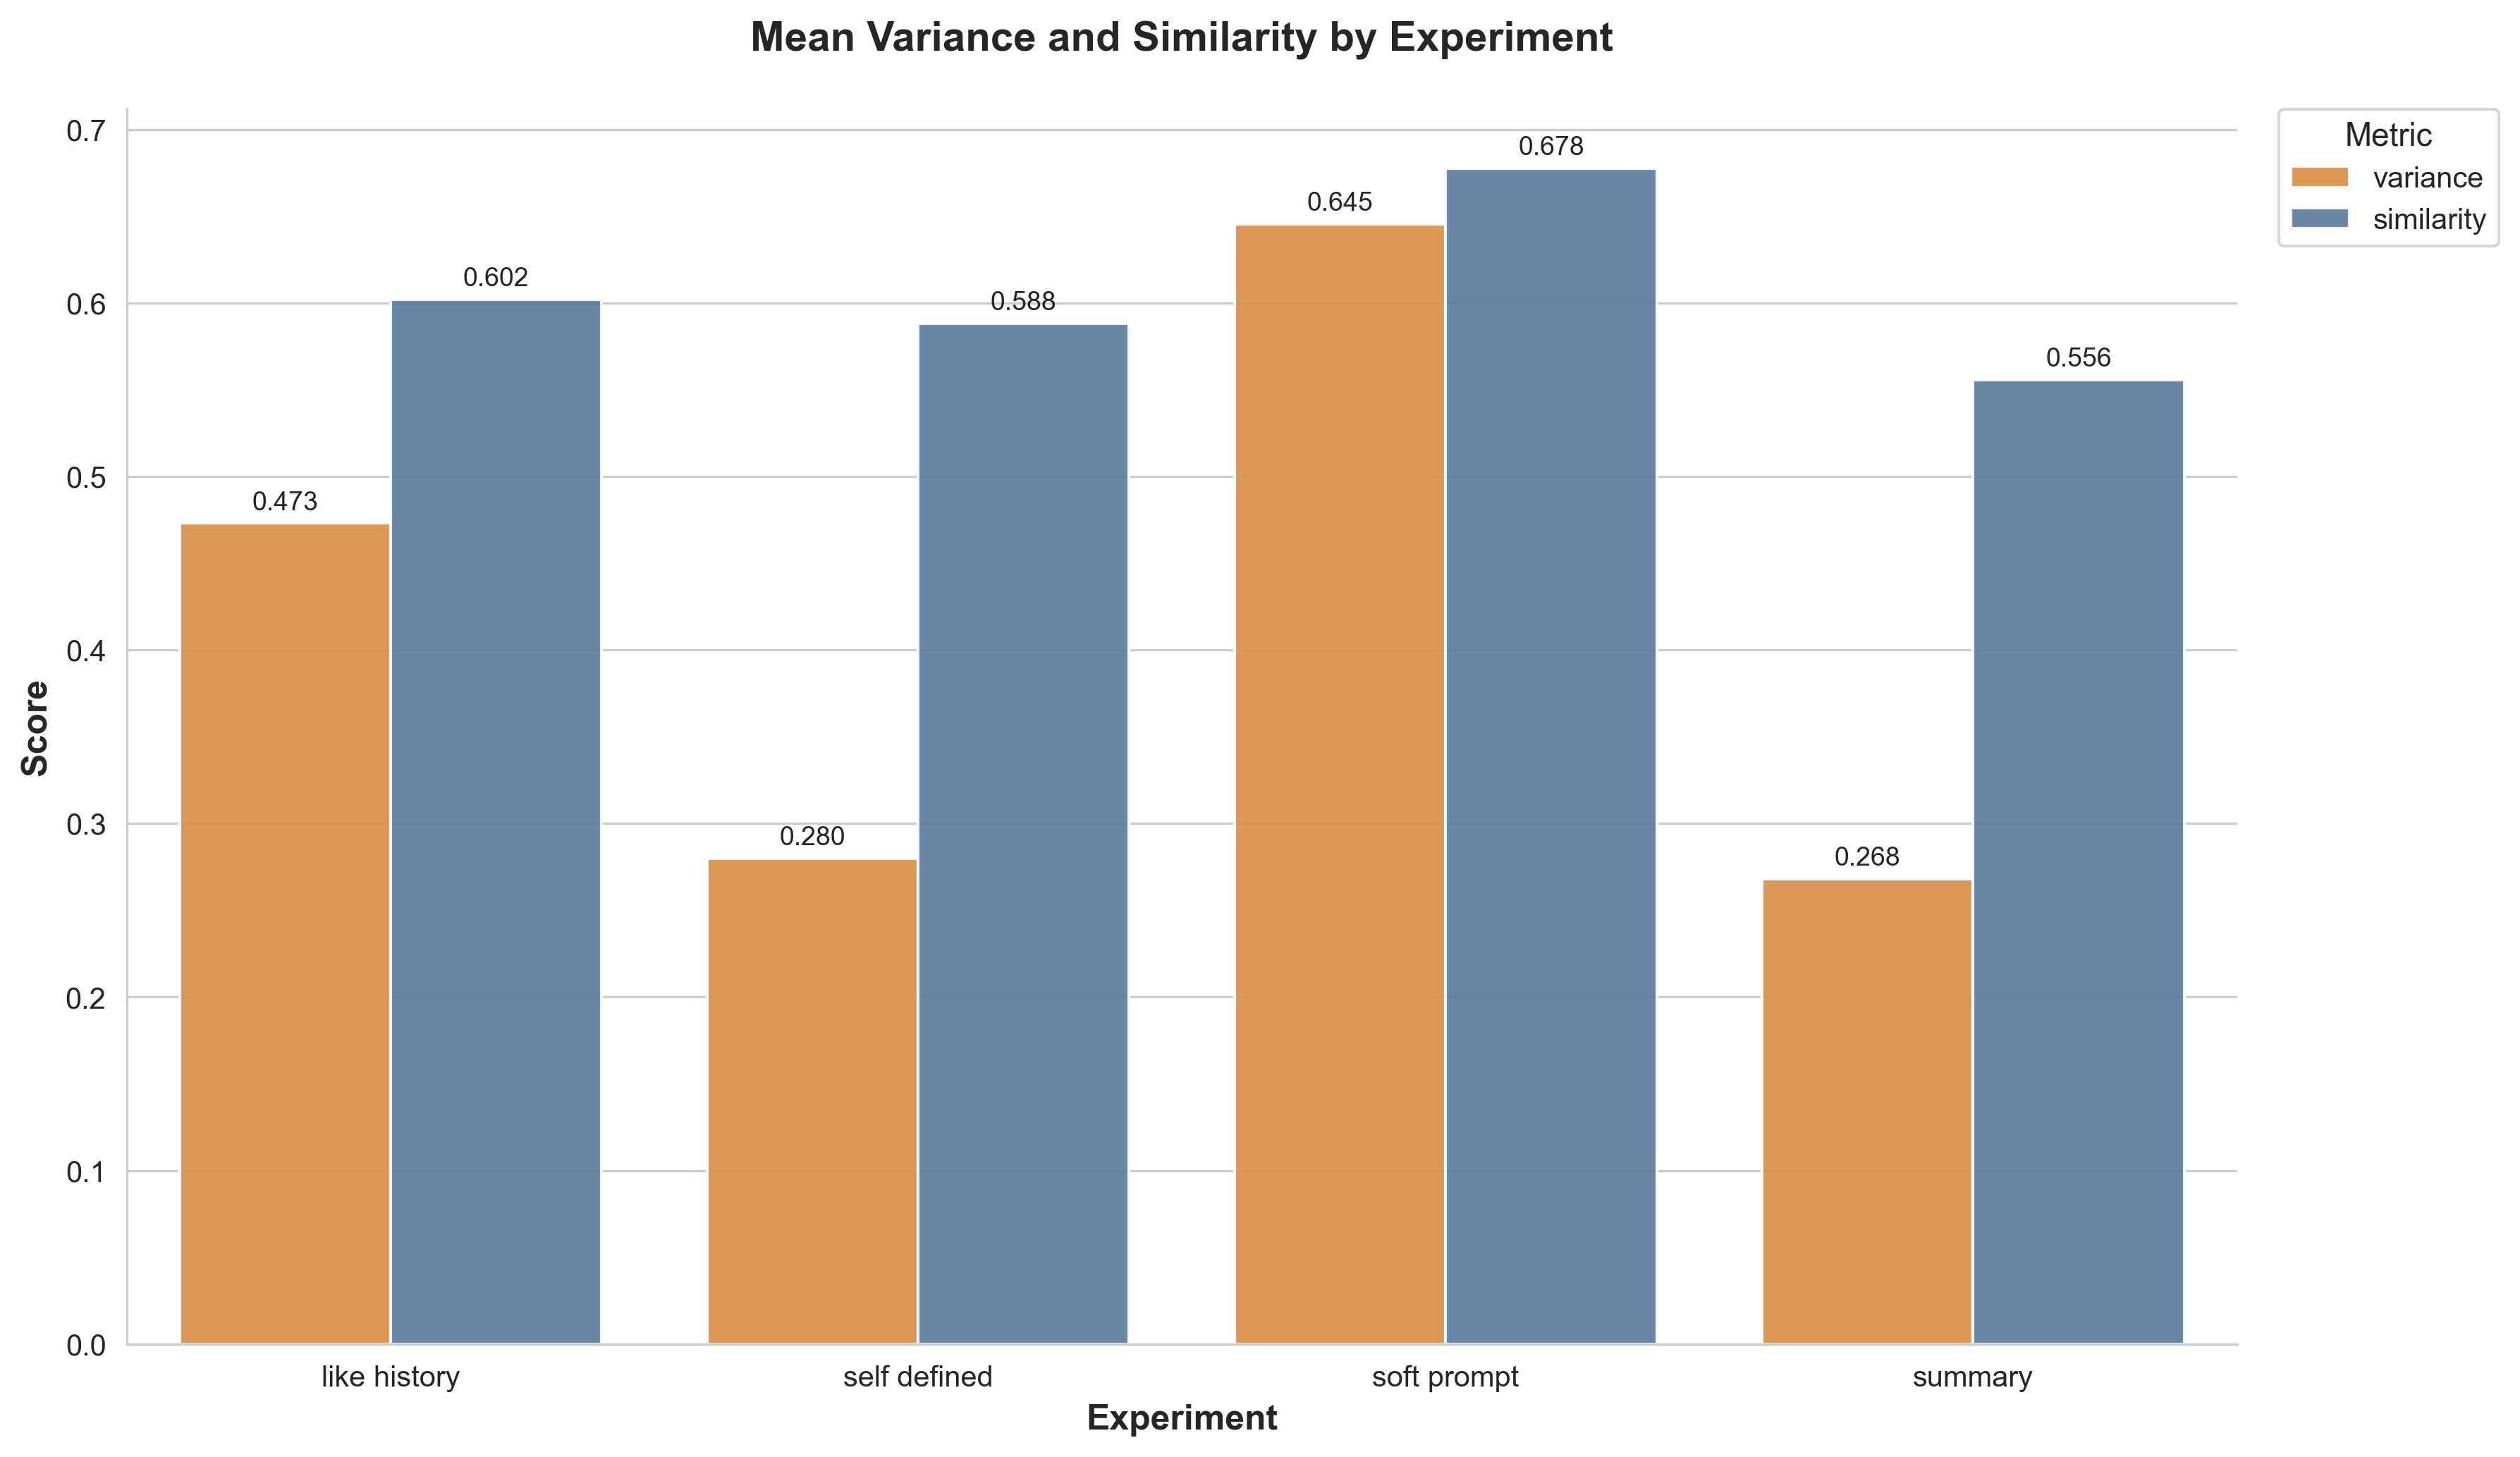
\includegraphics[width=\linewidth]{visuals/variance-similarity.png}
    \caption{}
    \label{fig:clustering-gemma-3-4b}
\end{figure}

\begin{figure}[h]
    \centering
    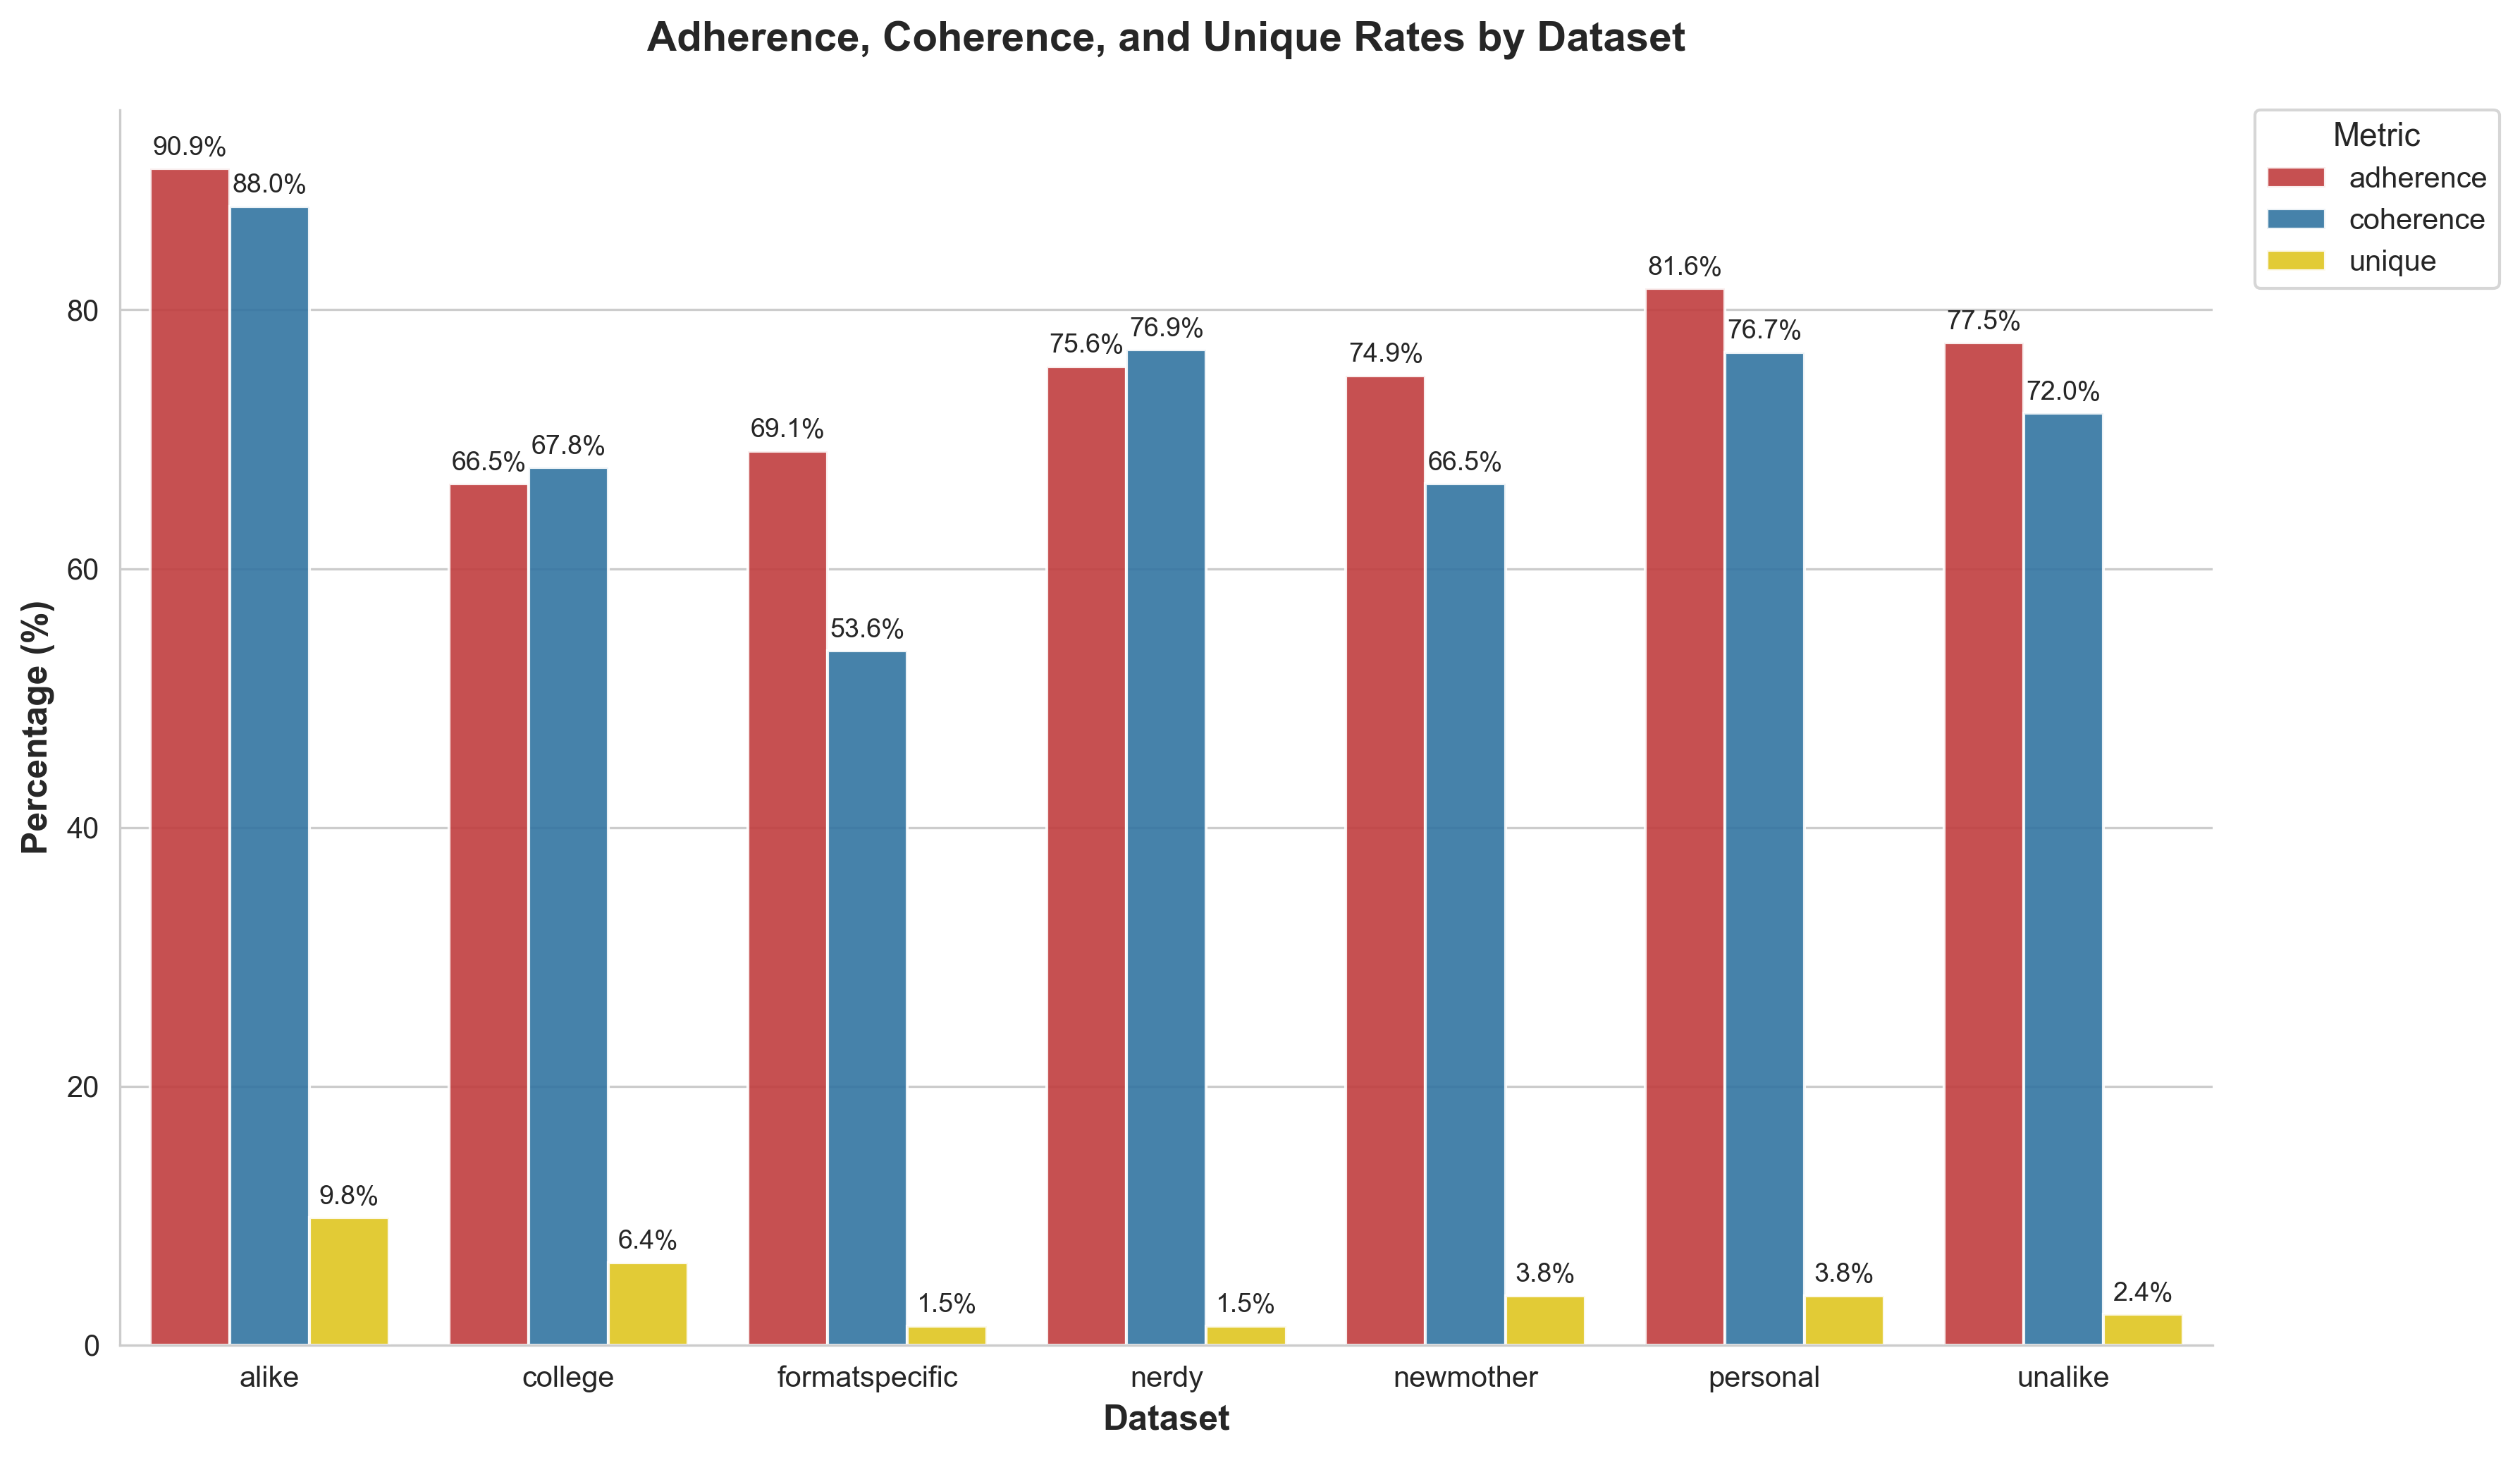
\includegraphics[width=\linewidth]{visuals/dataset-acu-rates.png}
    \caption{}
    \label{fig:clustering-gemma-3-4b}
\end{figure}

\begin{figure}[h]
    \centering
    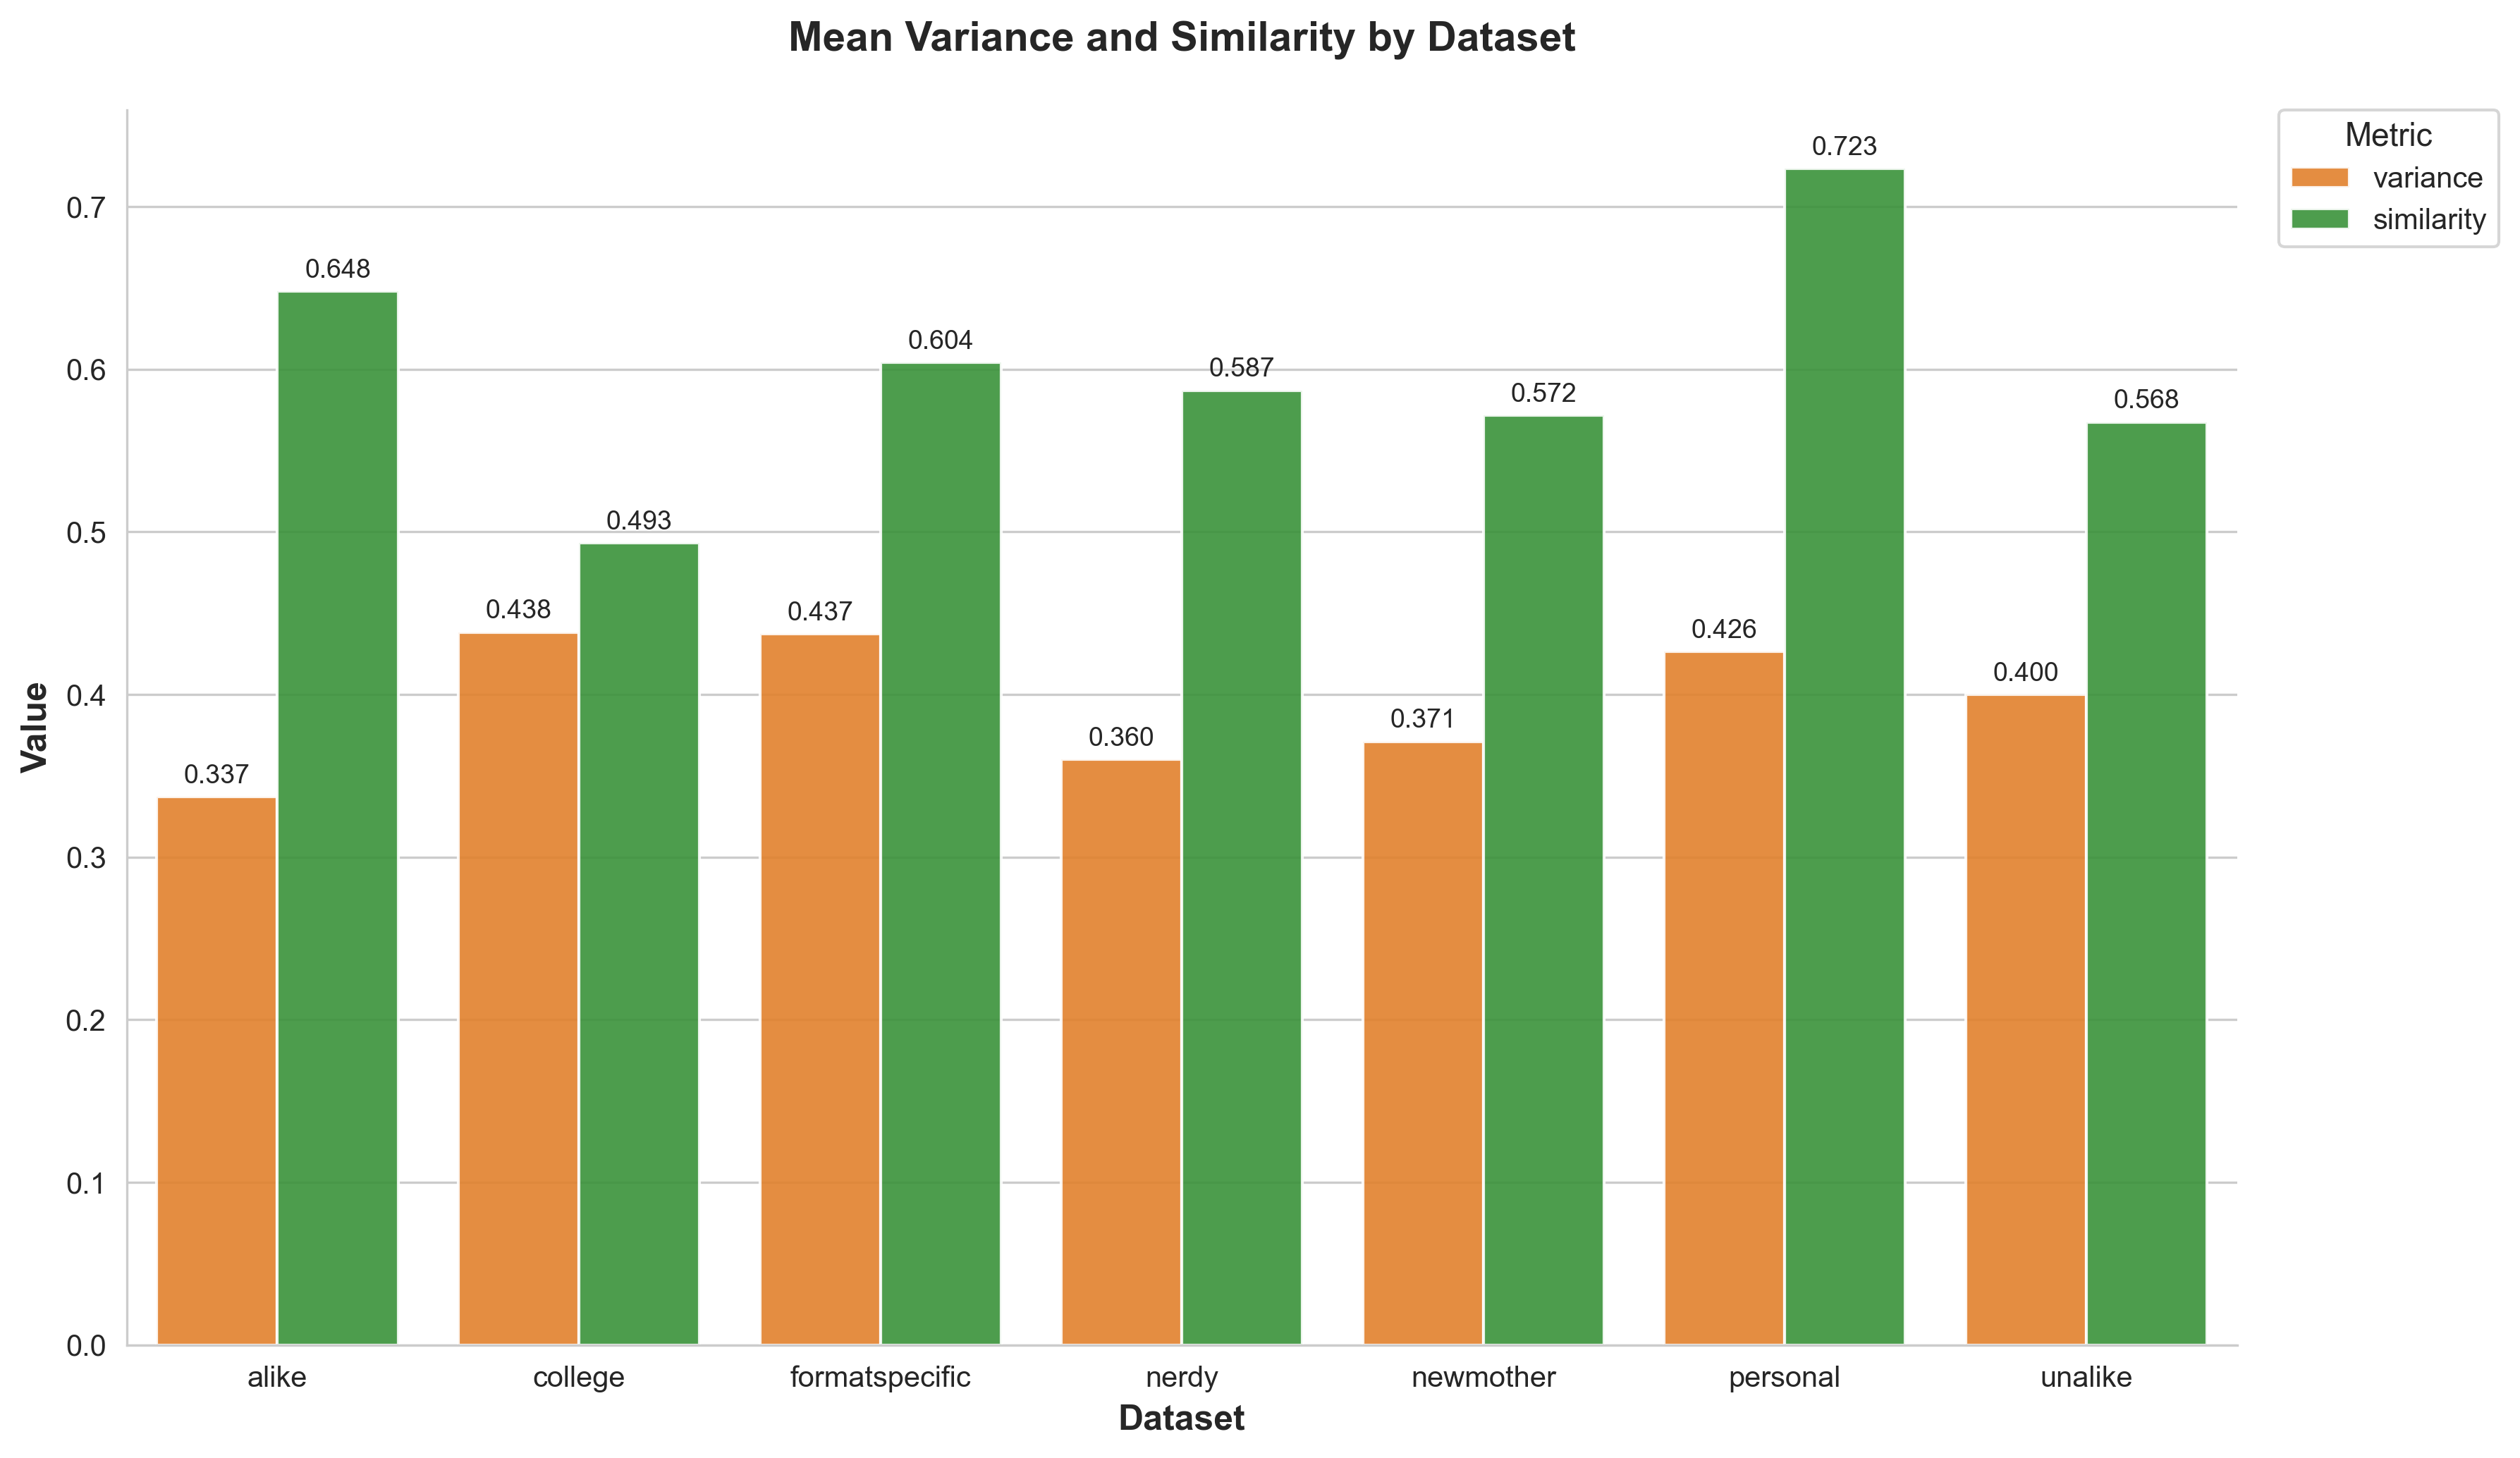
\includegraphics[width=\linewidth]{visuals/dataset-variance-similarity.png}
    \caption{}
    \label{fig:clustering-gemma-3-4b}
\end{figure}

\begin{figure}[h]
    \centering
    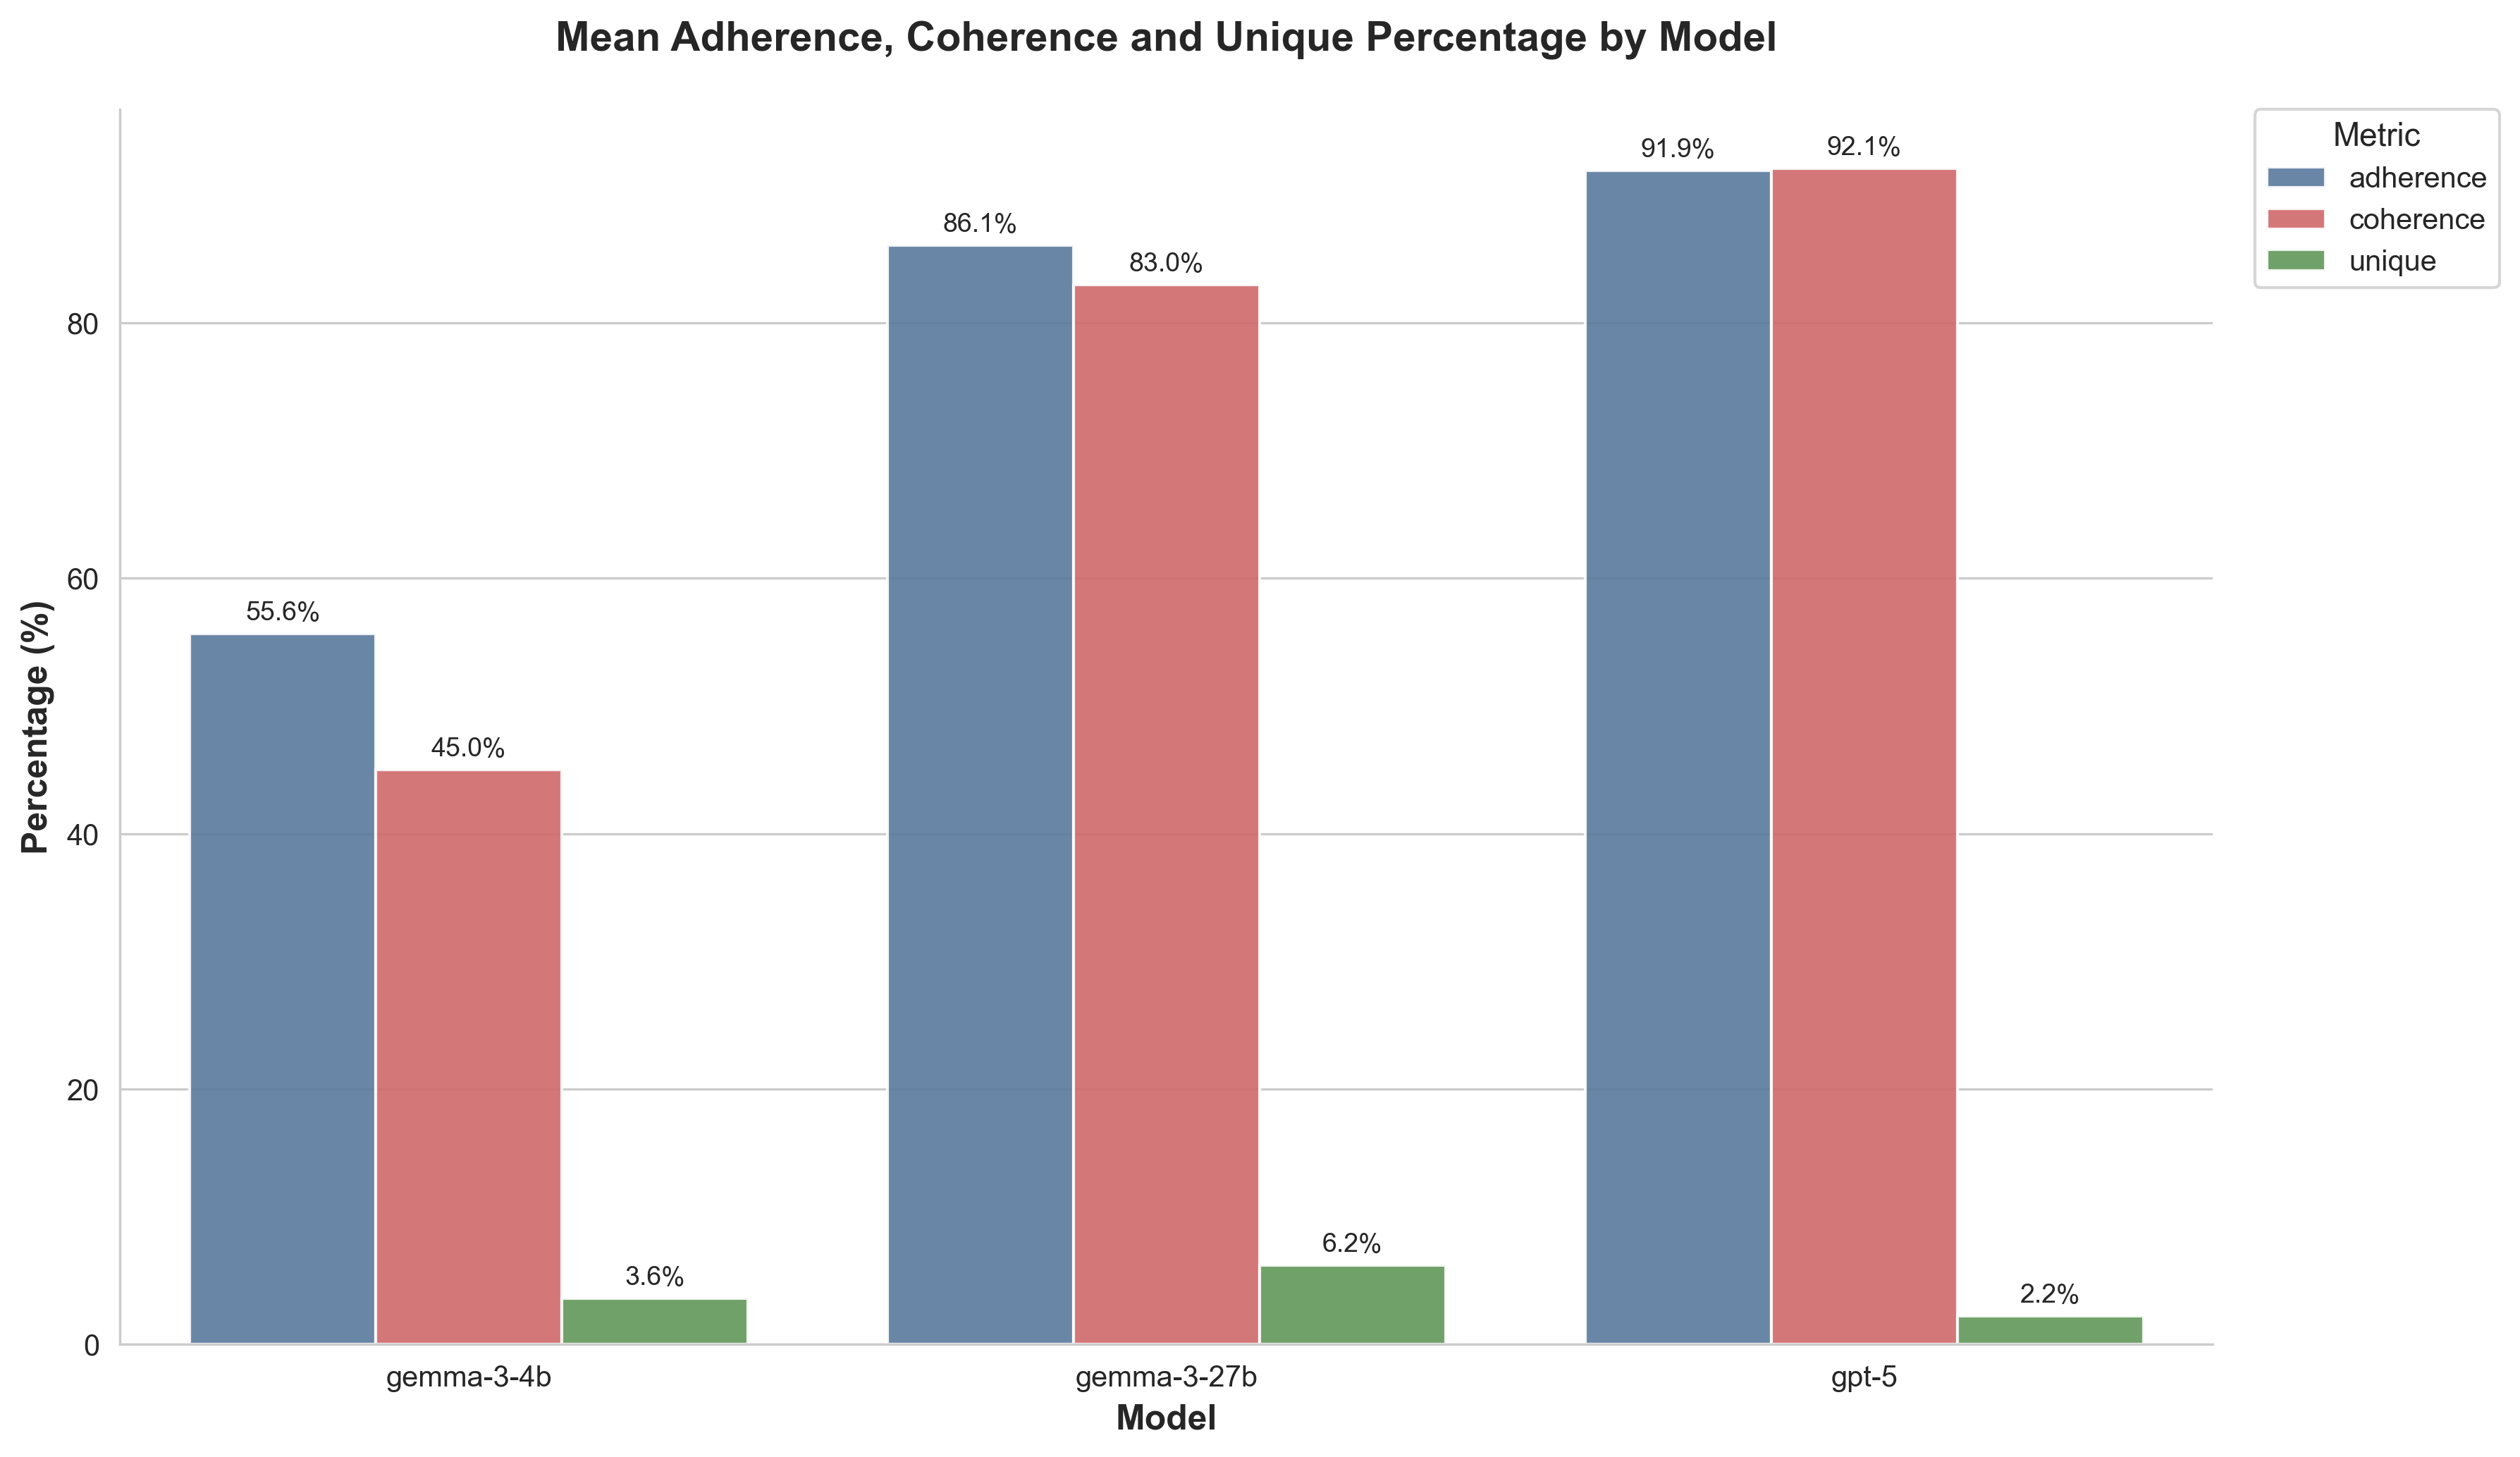
\includegraphics[width=\linewidth]{visuals/model-adherence-coherence-unique.png}
    \caption{}
    \label{fig:clustering-gemma-3-4b}
\end{figure}

\begin{figure}[h]
    \centering
    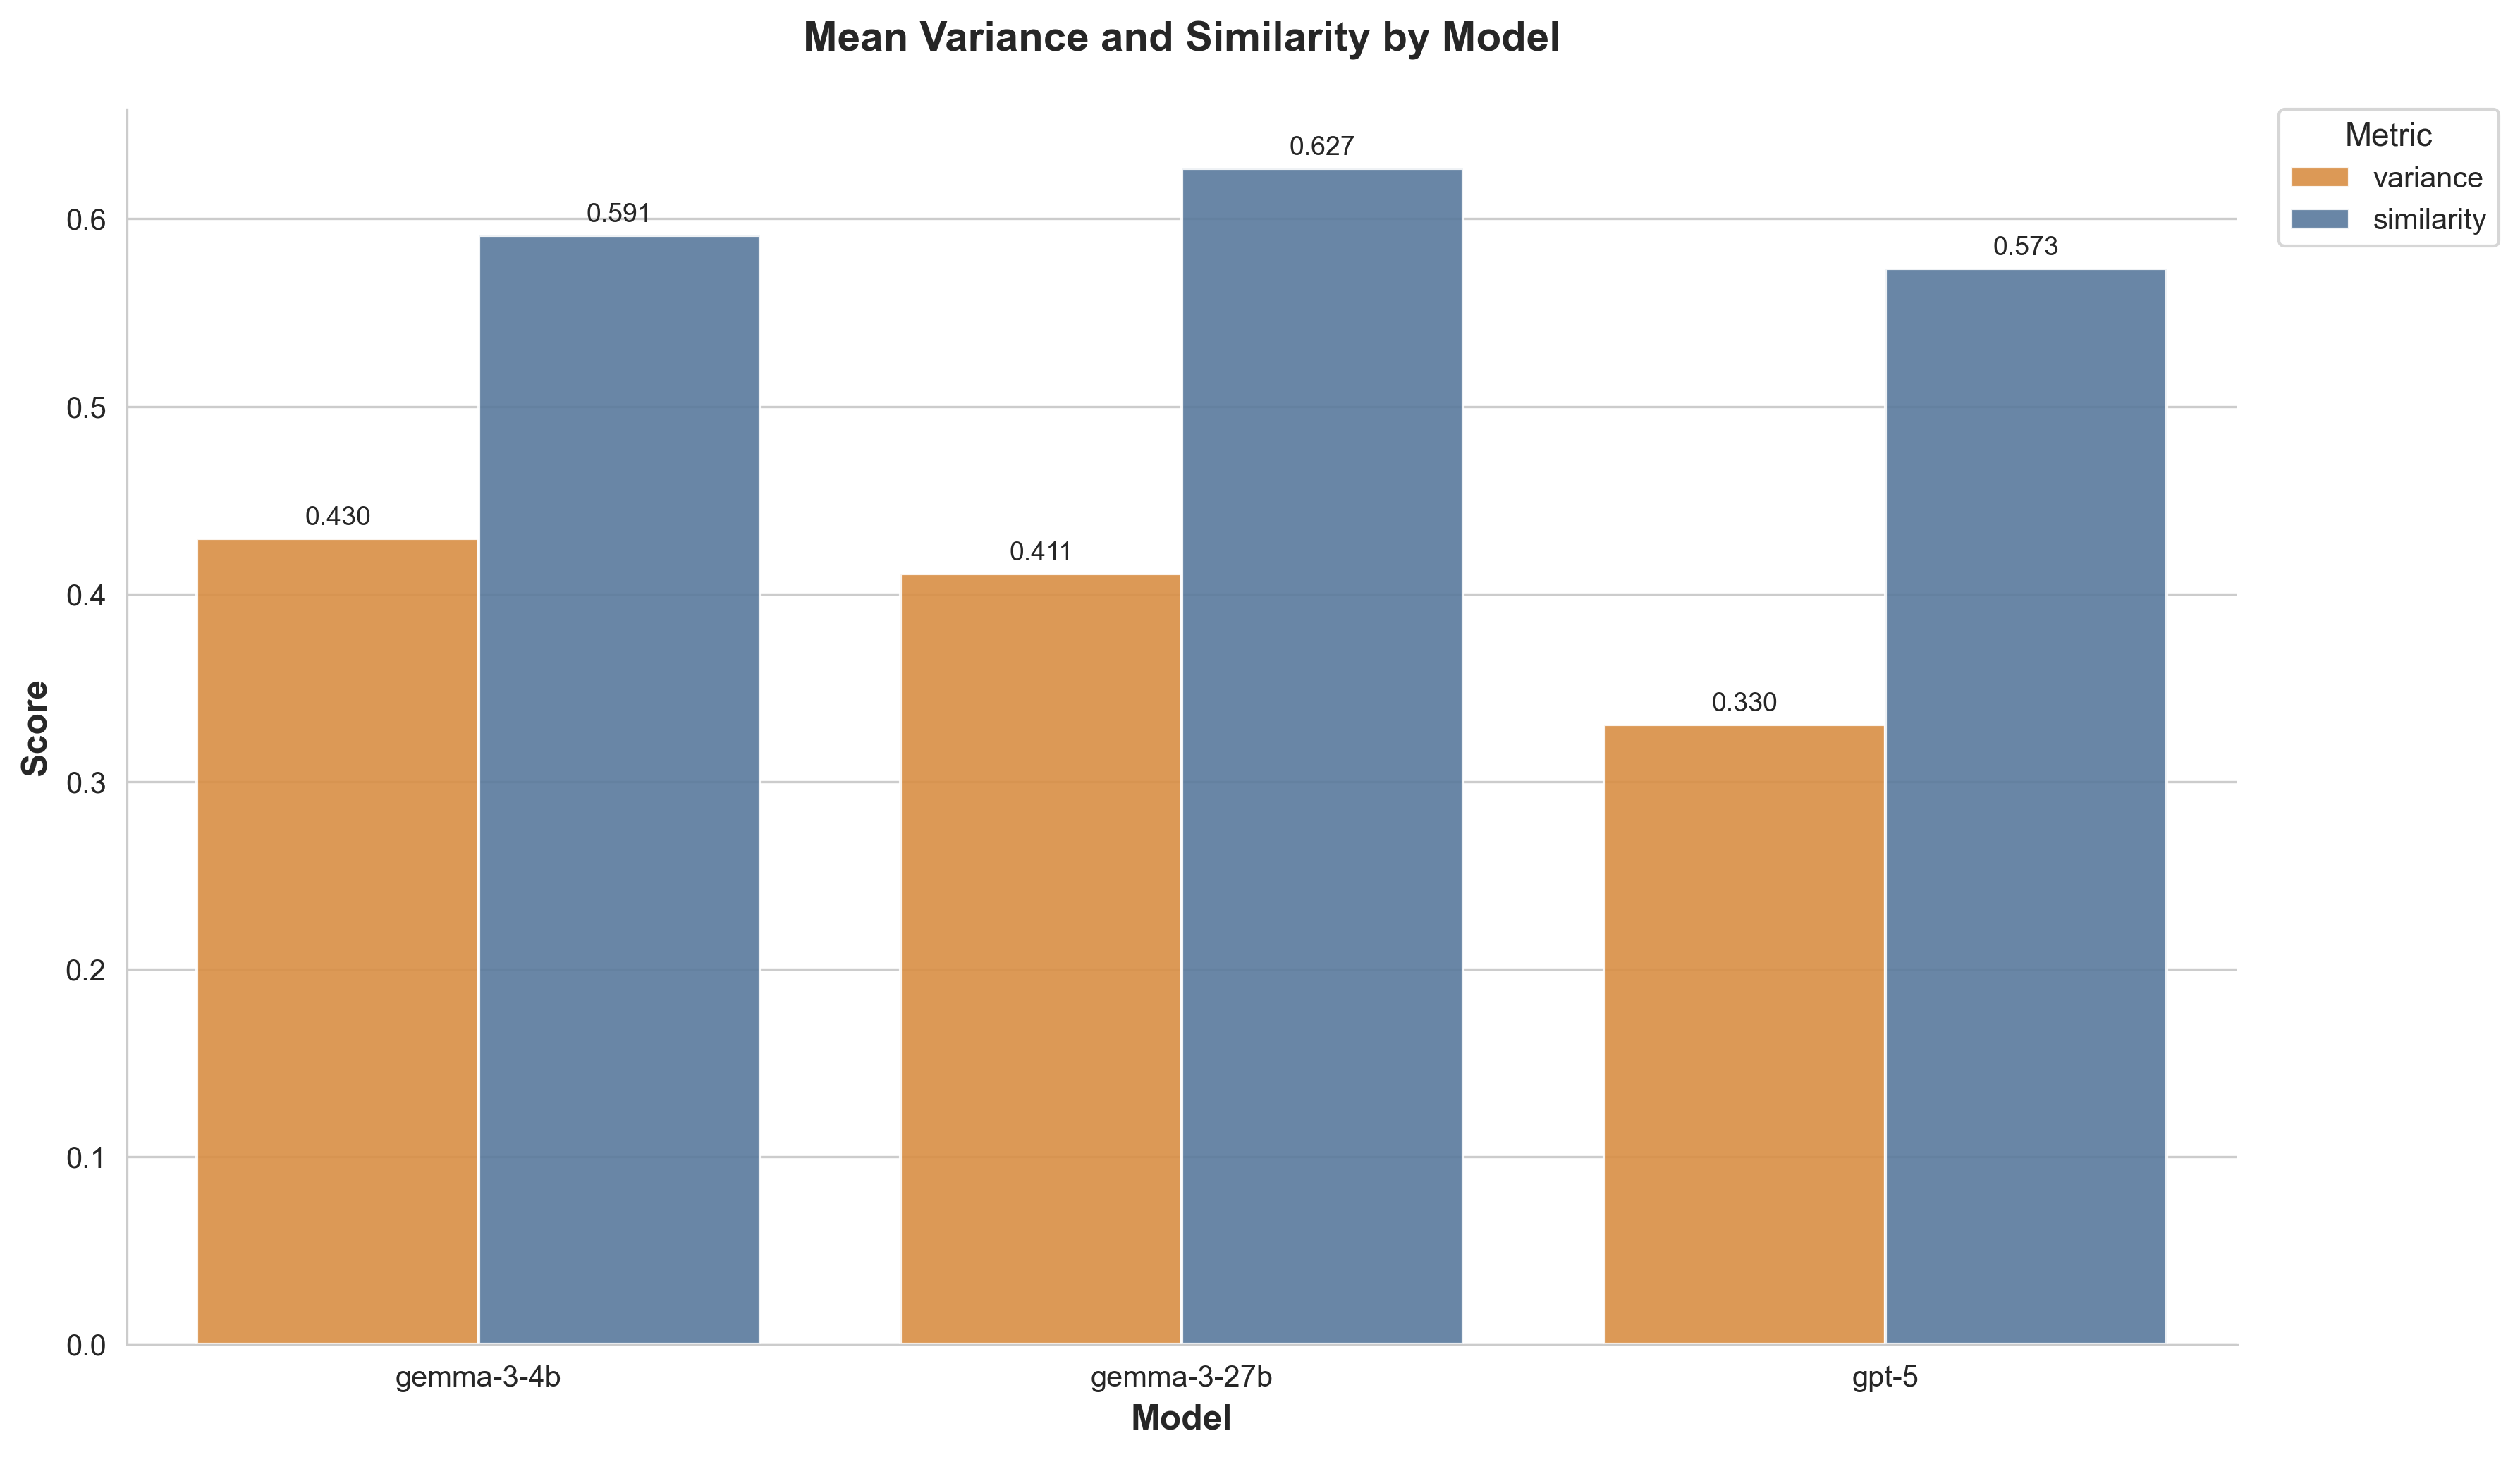
\includegraphics[width=\linewidth]{visuals/model-variance-similarity.png}
    \caption{}
    \label{fig:clustering-gemma-3-4b}
\end{figure}
\clearpage
\section{Appendix: Embedding Clustering}

\begin{figure}[h]
    \centering
    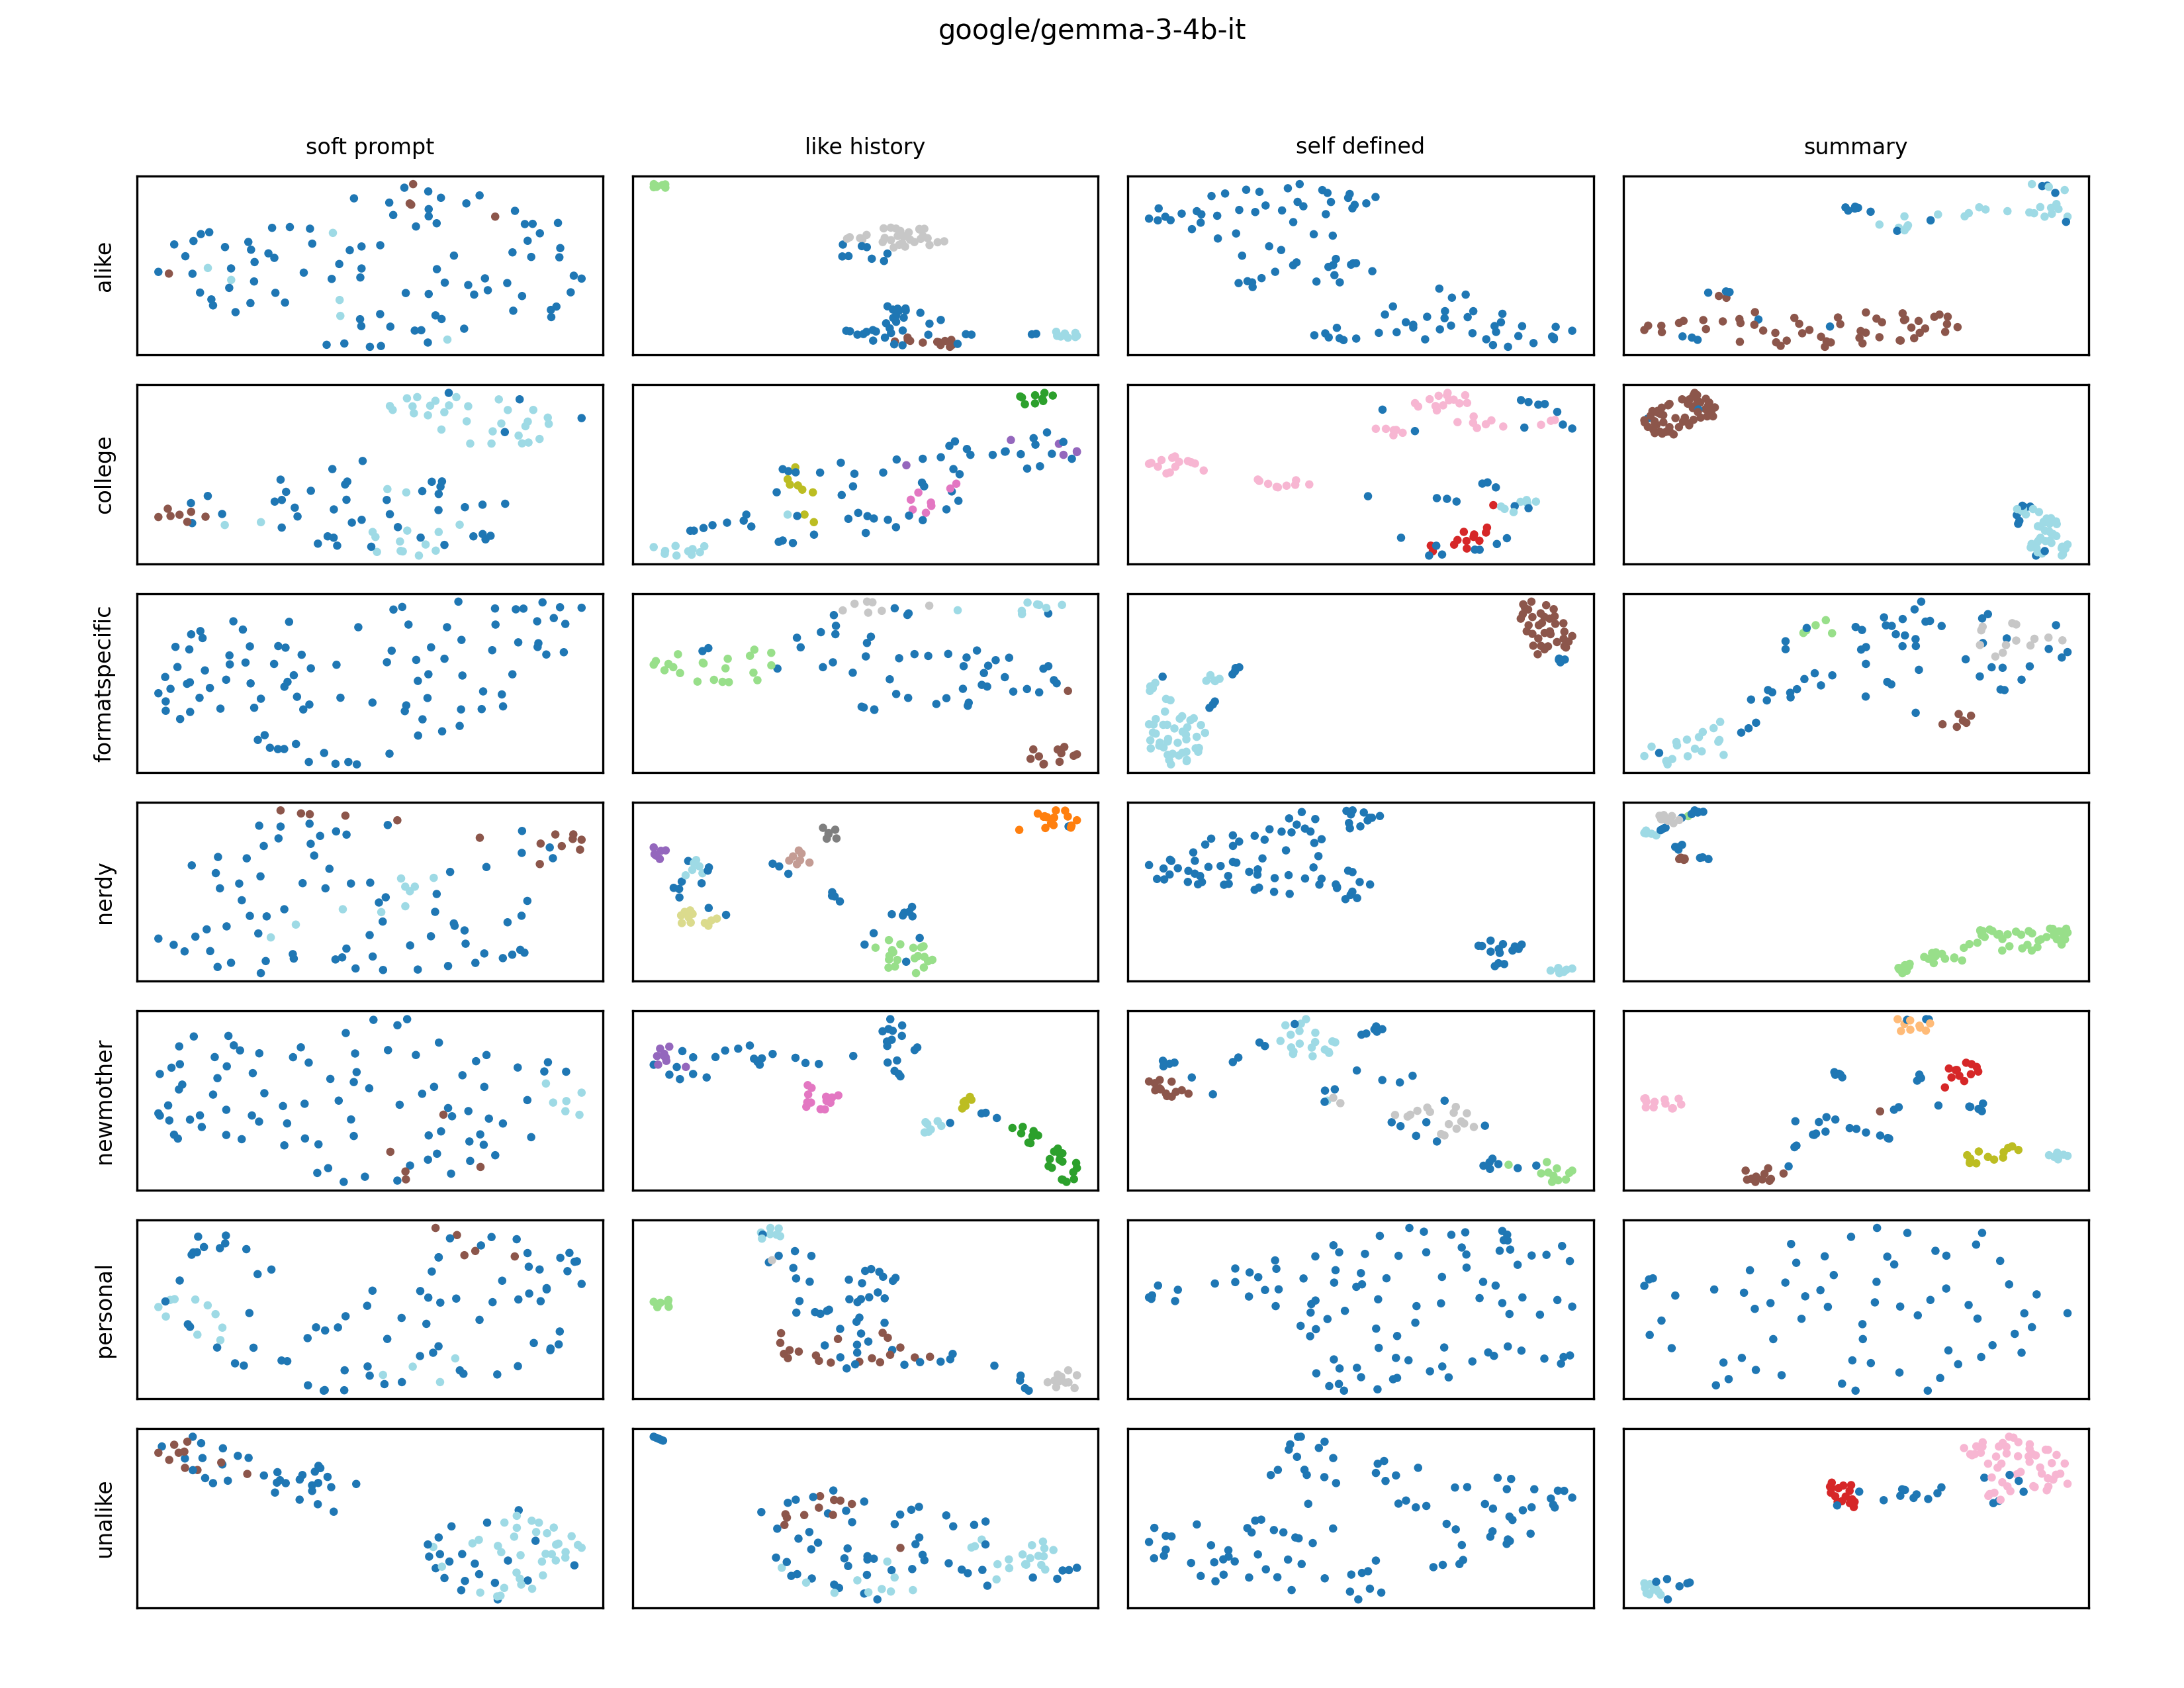
\includegraphics[width=\linewidth]{visuals/clustering/embeddings_google-gemma-3-4b-it_page_1}
    \caption{The clustering results show the large variety of posts that the soft prompt approach is able to generate. On the other hand, we see that summary is quite weak in this regard, often only generating small variations of the same 2 or 3 posts.}
    \label{fig:clustering-gemma-3-4b}
\end{figure}

\begin{figure}[h]
    \centering
    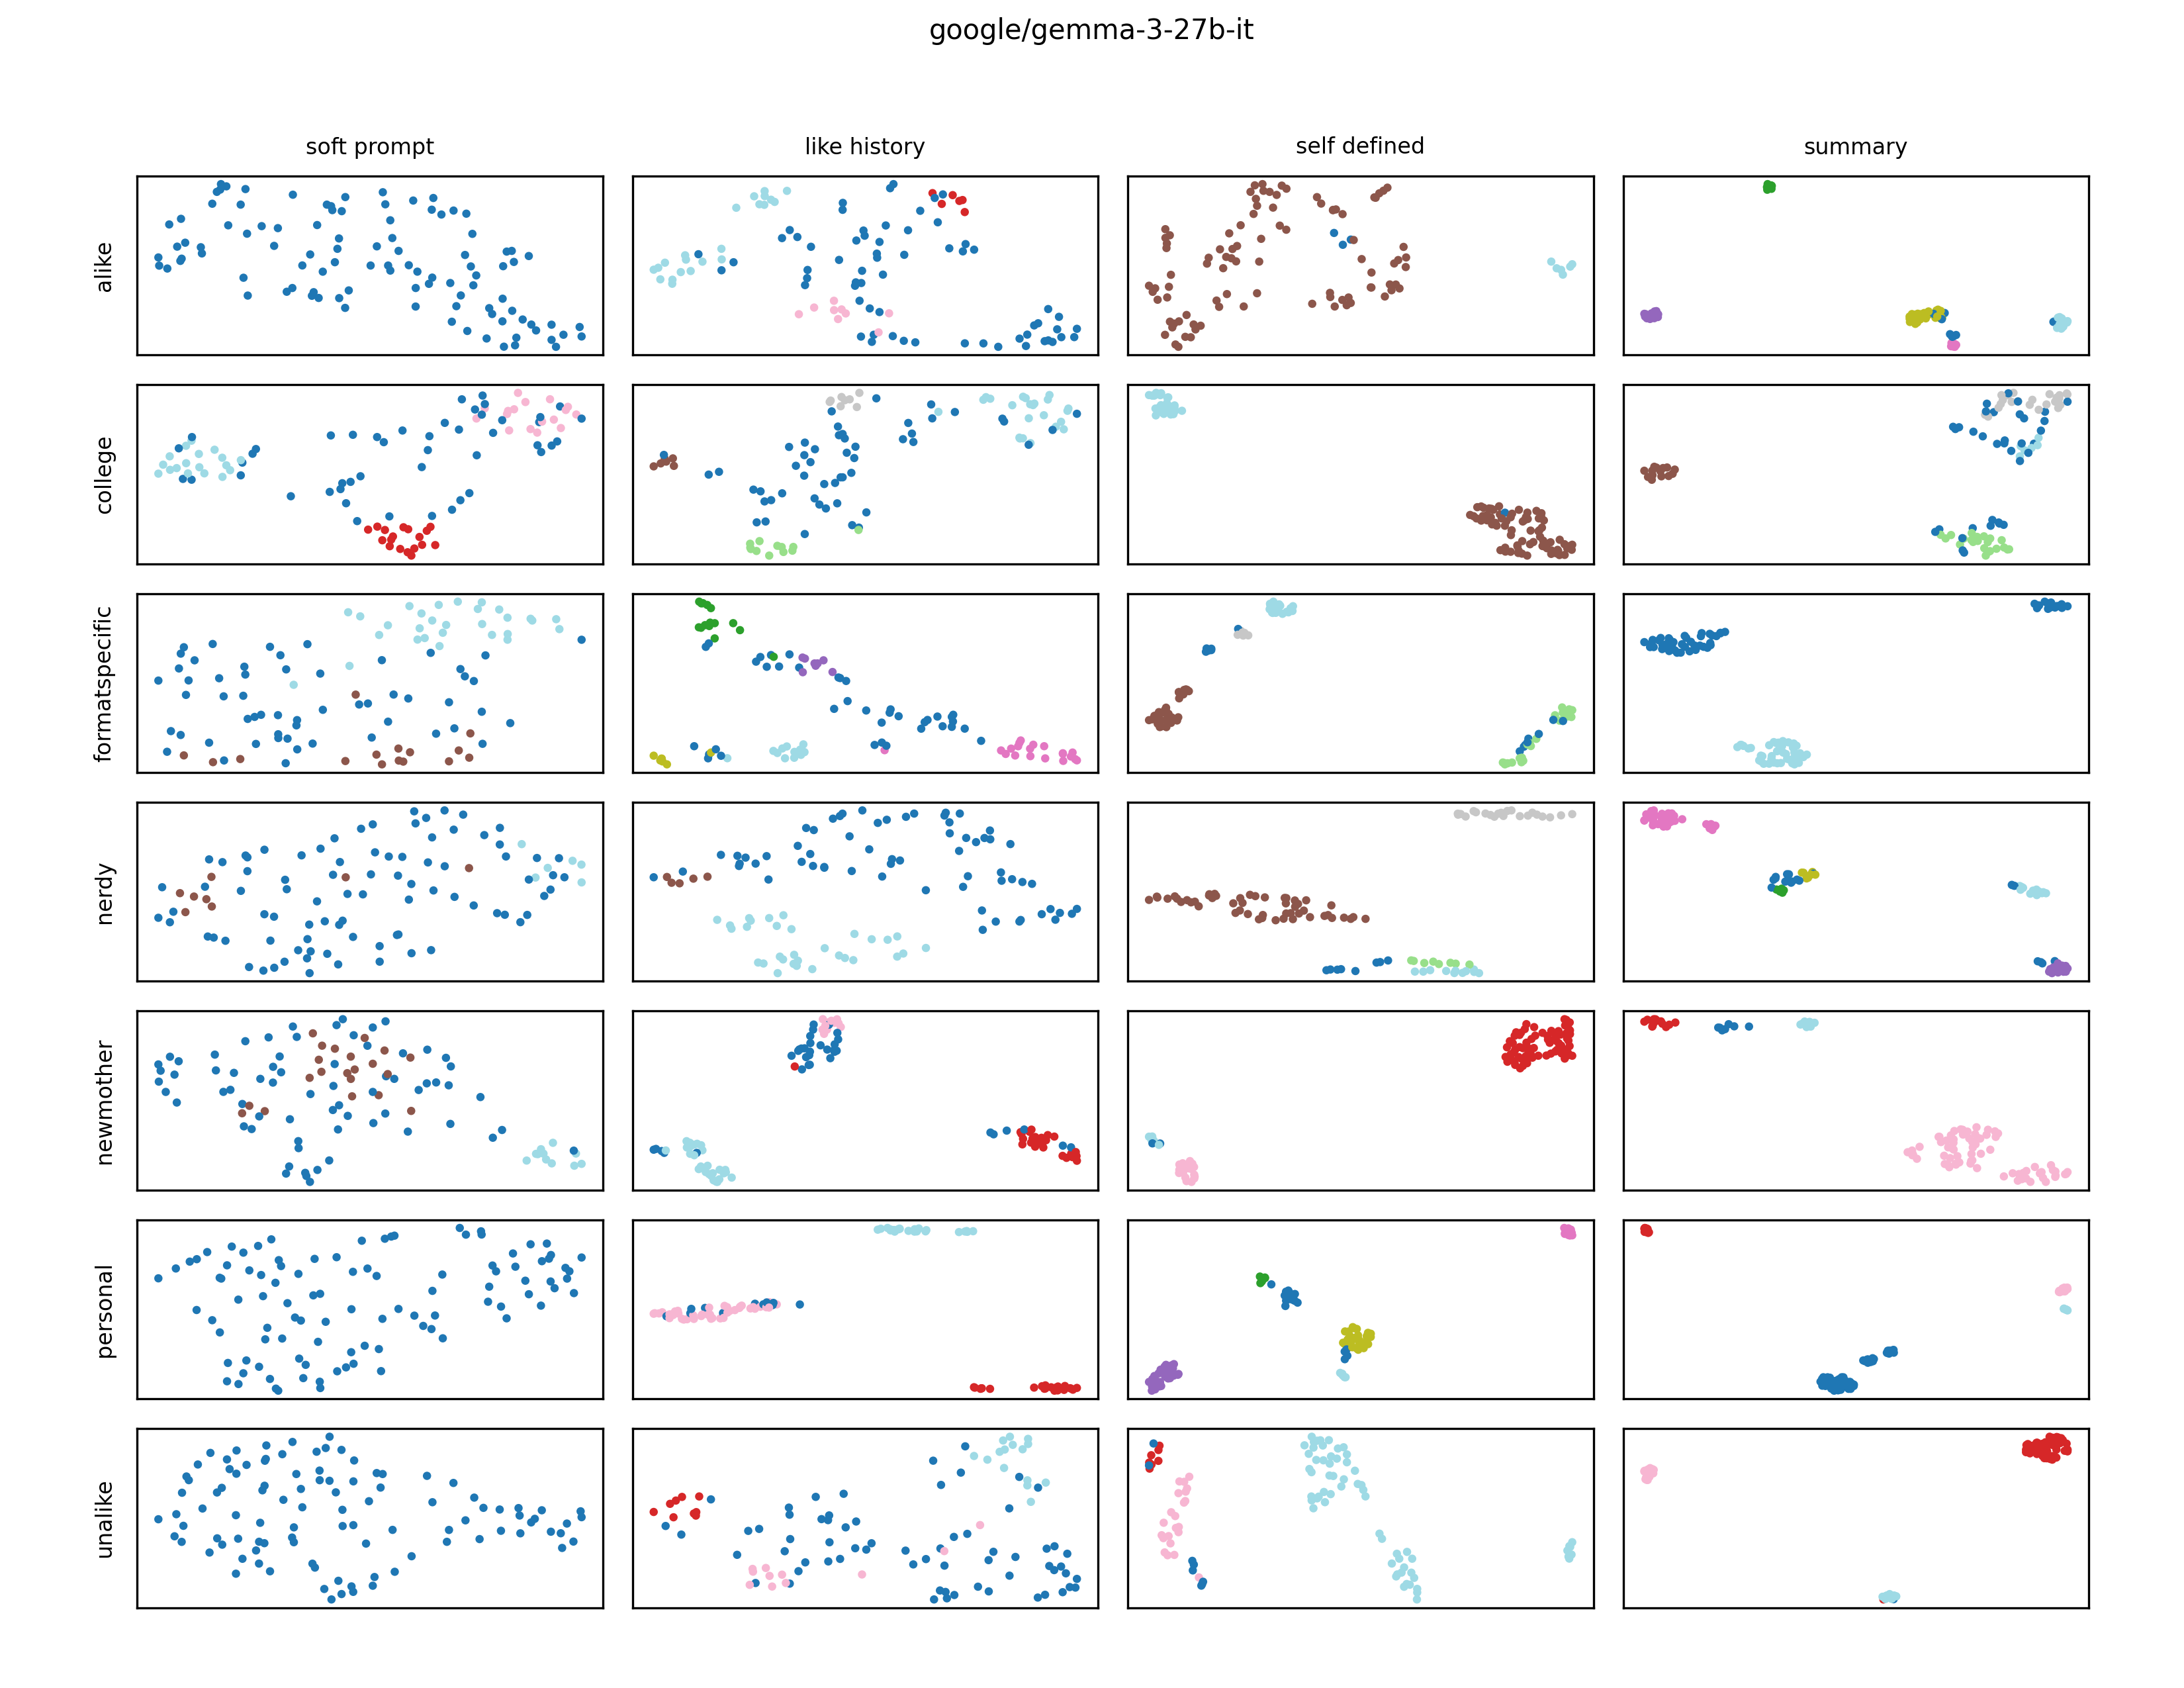
\includegraphics[width=\linewidth]{visuals/clustering/embeddings_google-gemma-3-27b-it_page_1}
    \caption{The clustering results show the large variety of posts that the soft prompt approach is able to generate. On the other hand, we see that summary is quite weak in this regard, often only generating small variations of the same 2 or 3 posts. Interestingly, this problem is even more pronounced for the larger model compared to its 4b counterpart.}
    \label{fig:clustering-gemma-3-27b}
\end{figure}

\begin{figure}[h]
    \centering
    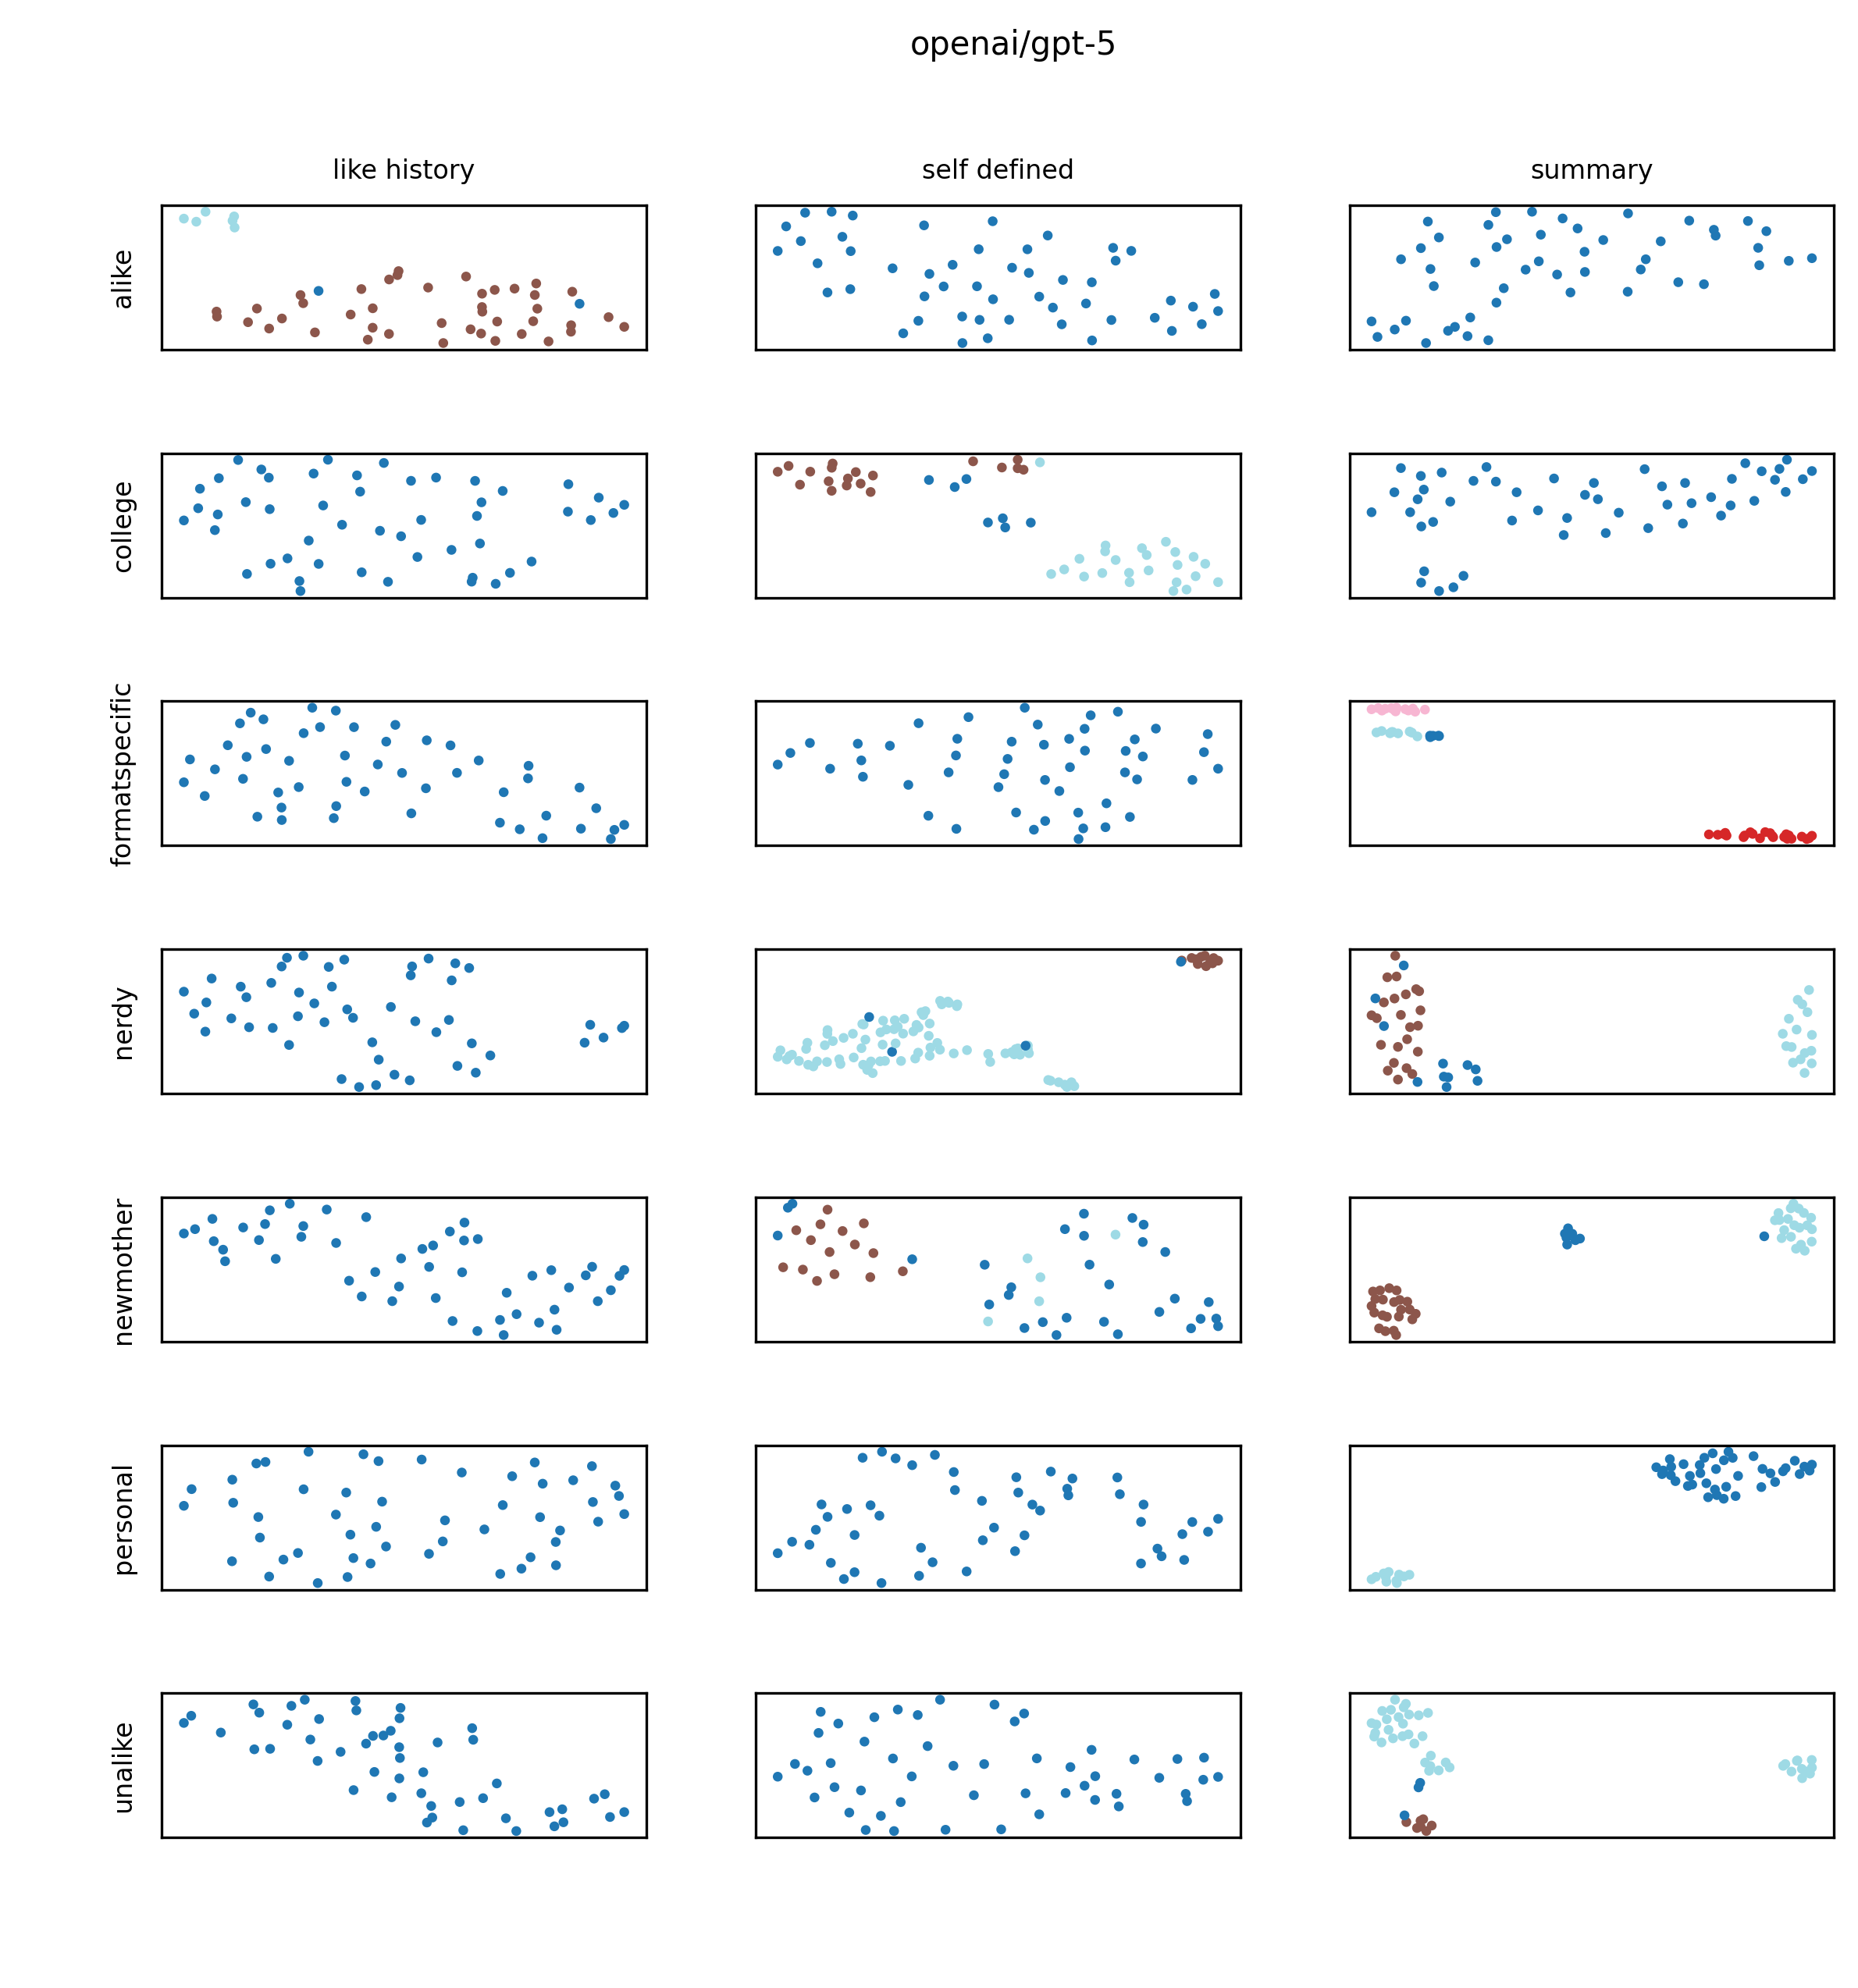
\includegraphics[width=\linewidth]{visuals/clustering/embeddings_openai-gpt-5_page_1}
    \caption{We see similar clustering results here, though not as pronounced as in the gemma models (in most cases).}
    \label{fig:clustering-gemma-3-4b}
\end{figure}

\end{document}
